\documentclass[12pt,a4paper]{article}
\usepackage[spanish]{babel}
\usepackage{geometry}
\usepackage{graphicx}
\usepackage{float}
\usepackage{amsmath}
\usepackage{amssymb}
\usepackage{hyperref}

\geometry{top=2.5cm, bottom=2.5cm, left=2.5cm, right=2.5cm}

\hypersetup{
    colorlinks=true,
    linkcolor=black,
    filecolor=magenta,      
    urlcolor=blue,
}

\begin{document}

\begin{titlepage}
    \centering
    \vspace*{1.5cm}
    
    
\includegraphics[width=8cm]{logoUGR.png}\par
    
    \vspace{3cm}
    
    {\Huge\bfseries \underline{MEMORIA DE PRÁCTICAS}\par}
    \vspace{0.4cm}
    {\Large\bfseries CURSO 2026/2027\par}
    \vspace{1cm}
    
    {\Large\itshape MODELOS DE COMPUTACIÓN\par}
    
    \vfill
    
    {\large\bfseries
    DIEGO DELGADO PÉREZ\par
    ADRIÁN VARELA JIMÉNEZ\par}
    
    \vspace{0.5cm}
    {\large Grupo C1\par}
    
    \vspace{2cm}
\end{titlepage}

\newpage
\tableofcontents
\newpage

\section{Práctica 1: Implementar un AFDM para verificar la parte del receptor en un protocolo de \mbox{comunicaciones}}

\subsection{Introducción y Motivación del Protocolo}
La validación de cadenas de datos es uno de los pilares fundamentales en el diseño de redes y comunicaciones. Desde la perspectiva de la Teoría de Autómatas y Lenguajes Formales, los paquetes de red pueden ser interpretados como palabras pertenecientes a un lenguaje regular (Tipo 3 en la Jerarquía de Chomsky), lo que permite que sean reconocidos y procesados por Autómatas Finitos con una eficiencia computacional máxima, operando en tiempo lineal $O(n)$ respecto a la longitud de la cadena.

En este contexto, y con el auge del Internet de las Cosas (IoT), los dispositivos periféricos operan frecuentemente alternando entre distintos modos de energía y prioridad de transmisión. El objetivo de esta práctica es diseñar, verificar formalmente y minimizar un Autómata Finito que modele el receptor de un protocolo de comunicación original diseñado para estos escenarios restrictivos. 

El sistema implementado ha sido bautizado como \textbf{Protocolo de Detección de Transición de Canal}. Este protocolo faculta al dispositivo receptor para discriminar instantáneamente si una trama entrante pertenece a un canal de telemetría de bajo consumo o a un canal de alerta crítica, exigiendo en ambos casos estrictas medidas de sincronización y un cierre seguro para evitar ataques de inyección o ruido en la línea.

El sistema opera sobre un alfabeto binario $\Sigma = \{0, 1\}$. Las reglas formales de aceptación que debe cumplir cualquier trama válida son las siguientes:
\begin{itemize}
    \item \textbf{Canal de Modo Eco (Inicia con 0):} La transmisión arranca con el bit `0`, lo que instruye al procesador a mantener un consumo energético mínimo. Para certificar la validez de la trama y evitar falsos positivos provocados por interferencias electromagnéticas, la secuencia debe contener obligatoriamente en su interior el patrón de sincronización \texttt{010}. Finalmente, el protocolo exige que la comunicación se cierre de manera estricta con el sufijo de control \textbf{\texttt{011}}.
    \item \textbf{Canal de Modo Alerta (Inicia con 1):} La transmisión arranca con el bit `1`, levantando una interrupción de alta prioridad en el receptor. En esta rama, la subsecuencia de sincronización exigida para validar la criticidad del mensaje es \texttt{101}. Al igual que en el modo anterior, el paquete de datos debe finalizar imperativamente con el sufijo de control \textbf{\texttt{011}} para que el autómata alcance un estado de aceptación.
\end{itemize}
Cualquier cadena que infrinja la correspondencia de los prefijos, que carezca de su respectivo patrón interno o que termine con una secuencia distinta al sufijo \texttt{011}, debe ser rechazada y descartada inmediatamente por el módulo receptor.

\newpage

\subsection{Diseño del Autómata Finito No Determinista (AFND)}
El primer paso en el flujo de diseño lógico del receptor ha consistido en la construcción de un Autómata Finito No Determinista (AFND). El uso del no determinismo representa una ventaja incalculable durante la fase de conceptualización humana, ya que permite modelar escenarios de bifurcación mediante transiciones nulas (transiciones $\lambda$ o $\epsilon$). Estas transiciones posibilitan que el autómata cambie de estado sin consumir ningún símbolo de la cadena de entrada, delegando en el sistema de cómputo subyacente la evaluación de múltiples caminos paralelos.

Para nuestro protocolo, el diseño parte de un estado inicial único que ejecuta dos transiciones $\lambda$ hacia sub-autómatas completamente independientes. La rama superior encapsula la lógica del Canal Eco, mientras que la rama inferior procesa el Canal de Alerta. Cada ruta ha sido dotada de:
\begin{enumerate}
    \item Un estado de lectura inicial condicionado (esperando `0` o `1`).
    \item Un bucle con transiciones \texttt{0,1} que actúa como sumidero para los bits de relleno pre-sincronización.
    \item Una concatenación lineal de estados que funciona como detector de subsecuencias para localizar los patrones \texttt{010} o \texttt{101}.
    \item Un segundo bucle de relleno para el cuerpo de la carga útil (payload).
    \item Una secuencia de salida terminal que exige la lectura exacta de los bits \texttt{0}, \texttt{1} y \texttt{1} para culminar en el estado de aceptación final.
\end{enumerate}

\begin{figure}[H]
    \centering
    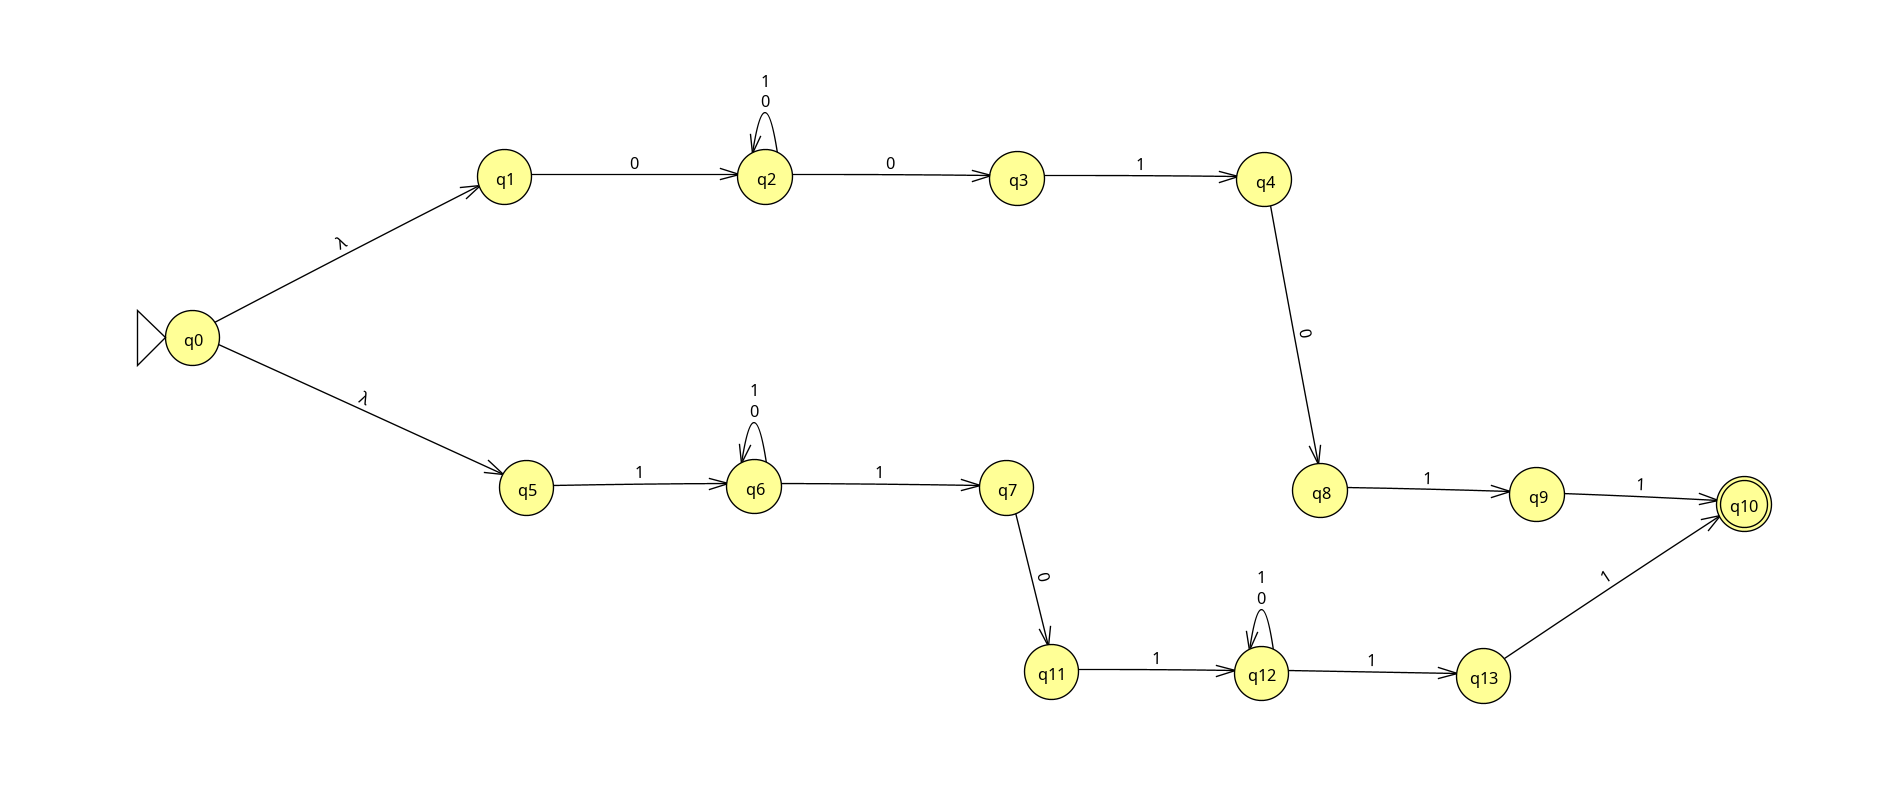
\includegraphics[width=0.85\textwidth]{../P1/img/afnd_diseño.png}
    \caption{Arquitectura del AFND empleando transiciones $\lambda$ para la bifurcación semántica inicial en JFLAP.}
    \label{fig:afnd_diseno}
\end{figure}

\subsubsection{Verificación Experimental del AFND}
Todo diseño abstracto requiere validación empírica. Mediante la herramienta \textit{Multiple Run} del entorno JFLAP, se ha sometido al autómata a un riguroso banco de pruebas. Se han introducido tanto cadenas de control positivas (que cumplen íntegramente las especificaciones de sus respectivos canales) como cadenas negativas (diseñadas para fallar en el sufijo, confundir el patrón intermedio o iniciar con un bit que no corresponde a la rama evaluada).

\begin{figure}[H]
    \centering
    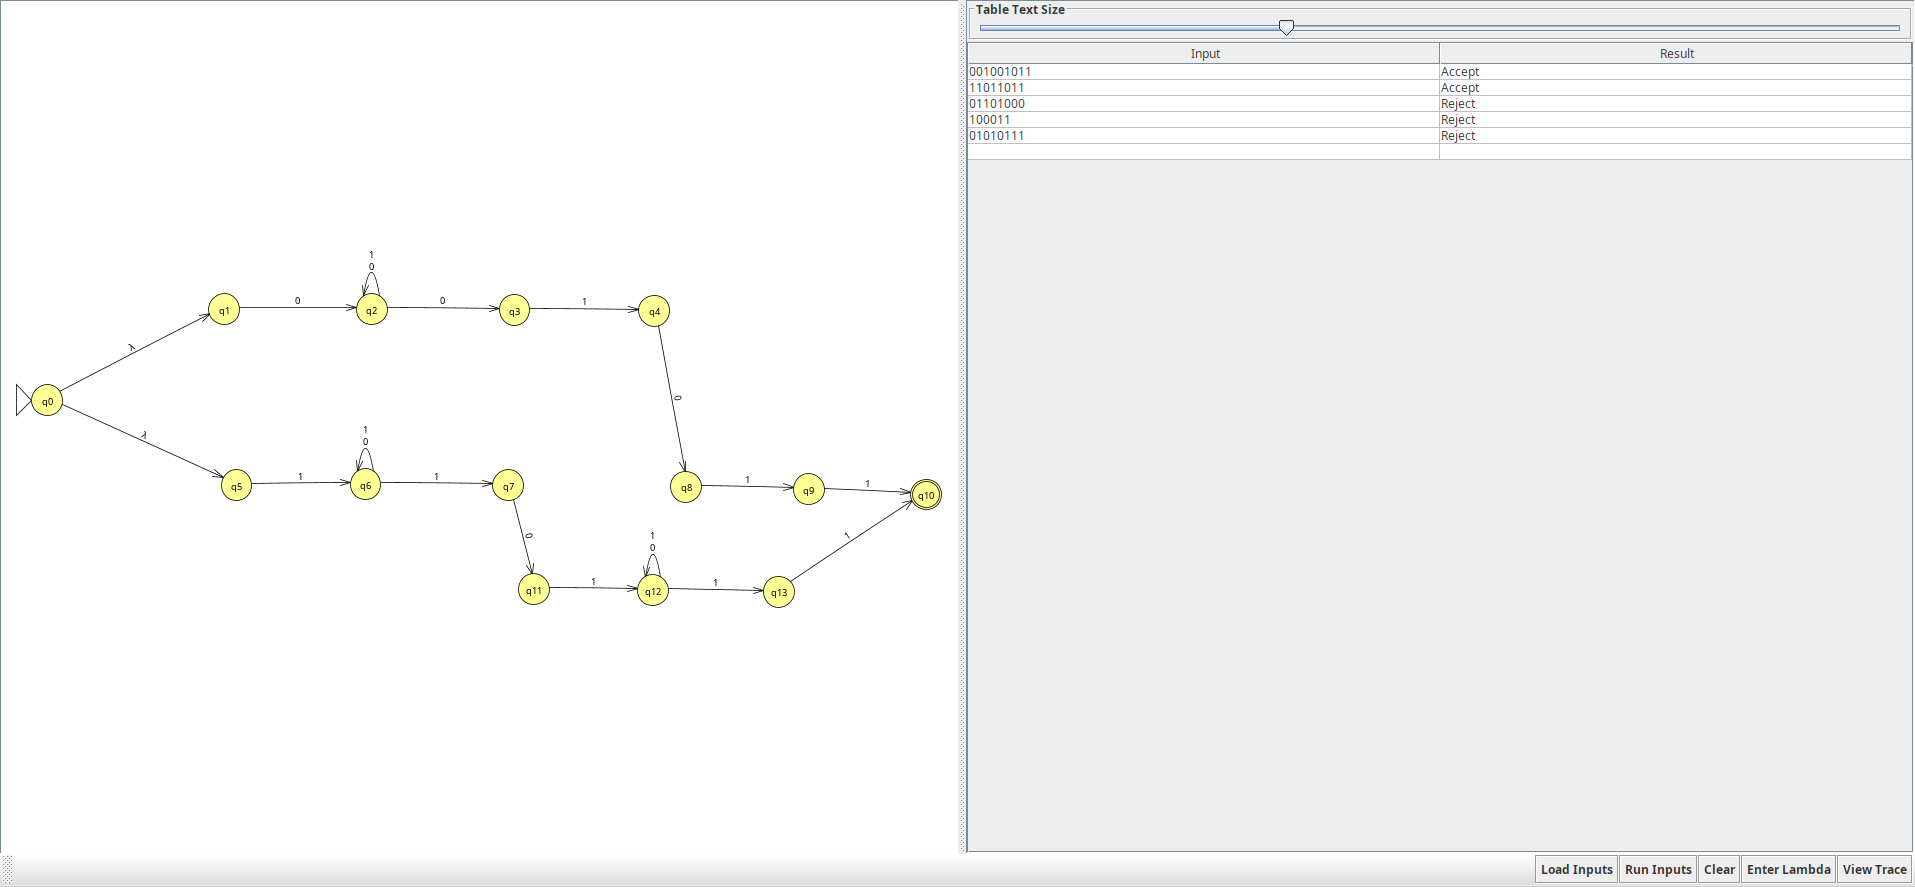
\includegraphics[width=0.85\textwidth]{../P1/img/afnd_tests.png}
    \caption{Validación exhaustiva de las tramas mediante múltiples ejecuciones. Se certifica empíricamente que los rechazos y aceptaciones coinciden al 100\% con la lógica de negocio del protocolo.}
    \label{fig:afnd_tests}
\end{figure}

\vspace{1cm}

El análisis de las trazas de ejecución permite visualizar el comportamiento interno del algoritmo de retroceso (backtracking) de JFLAP, ilustrando cómo los hilos de procesamiento no válidos mueren al no encontrar transiciones lícitas, sobreviviendo únicamente el camino que conduce al estado de aceptación si la trama es sintácticamente correcta.

\vspace{1cm}

\begin{figure}[H]
    \centering
    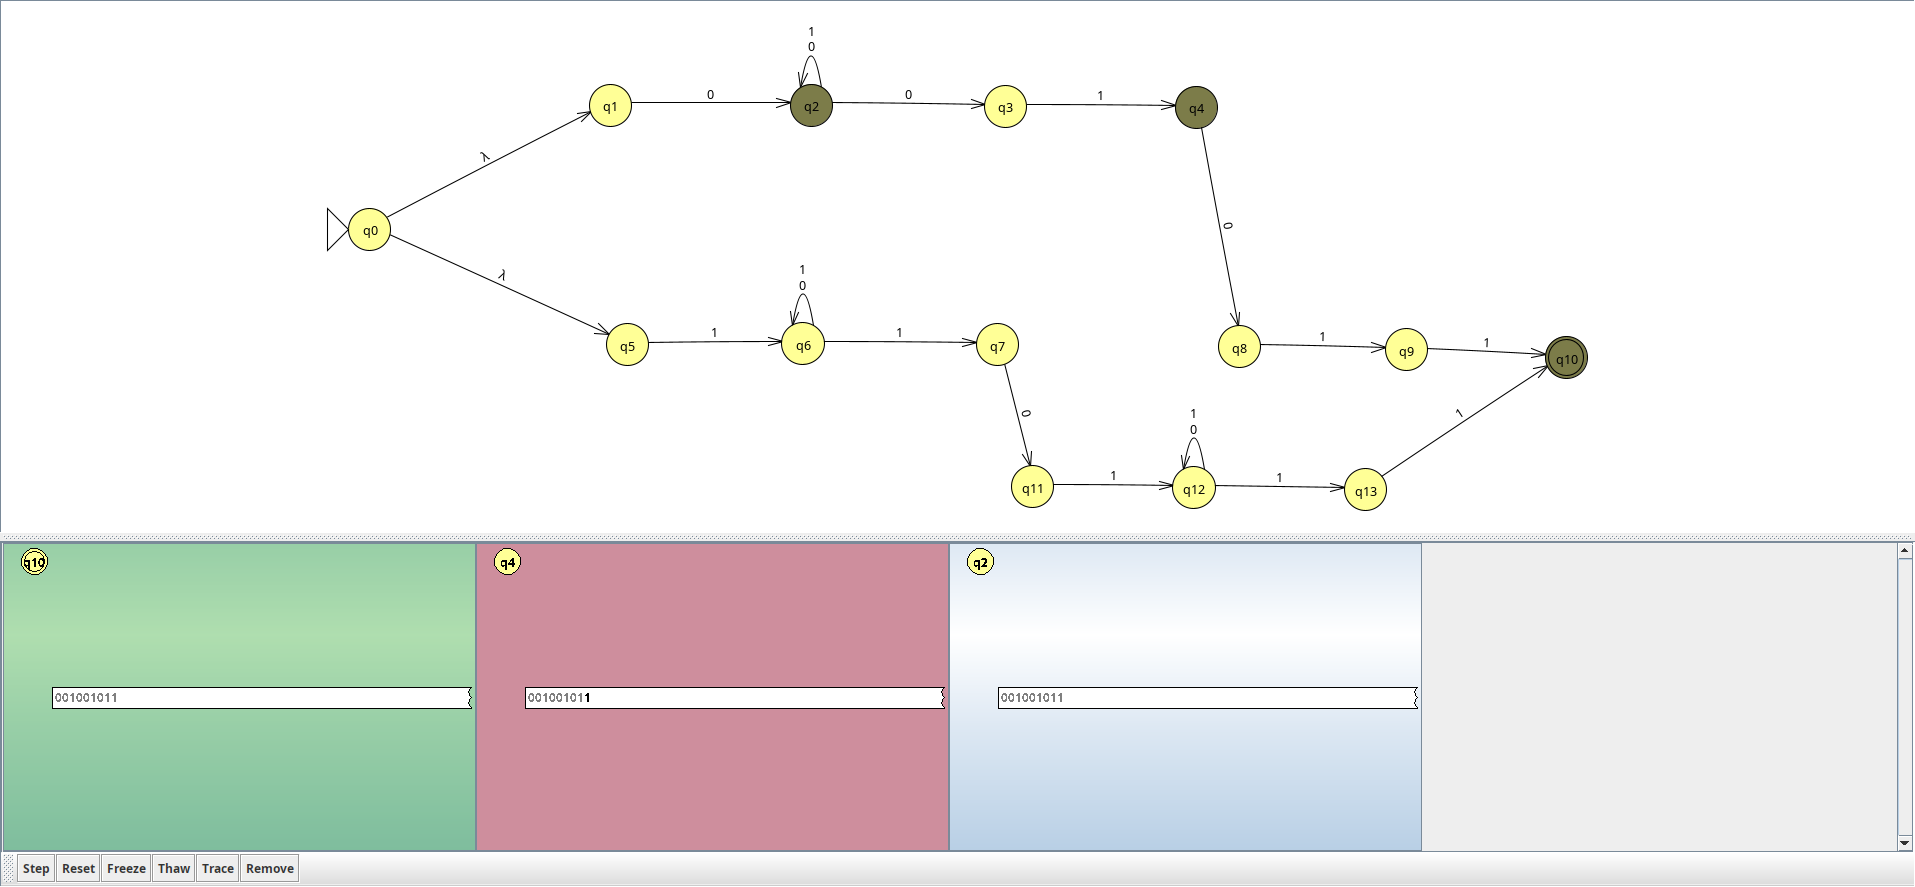
\includegraphics[width=0.85\textwidth]{../P1/img/traza_1.png}
    \caption{Procesamiento de una trama válida (Traza 1) resolviendo el no determinismo.}
    \label{fig:traza_1}
\end{figure}

\begin{figure}[H]
    \centering
    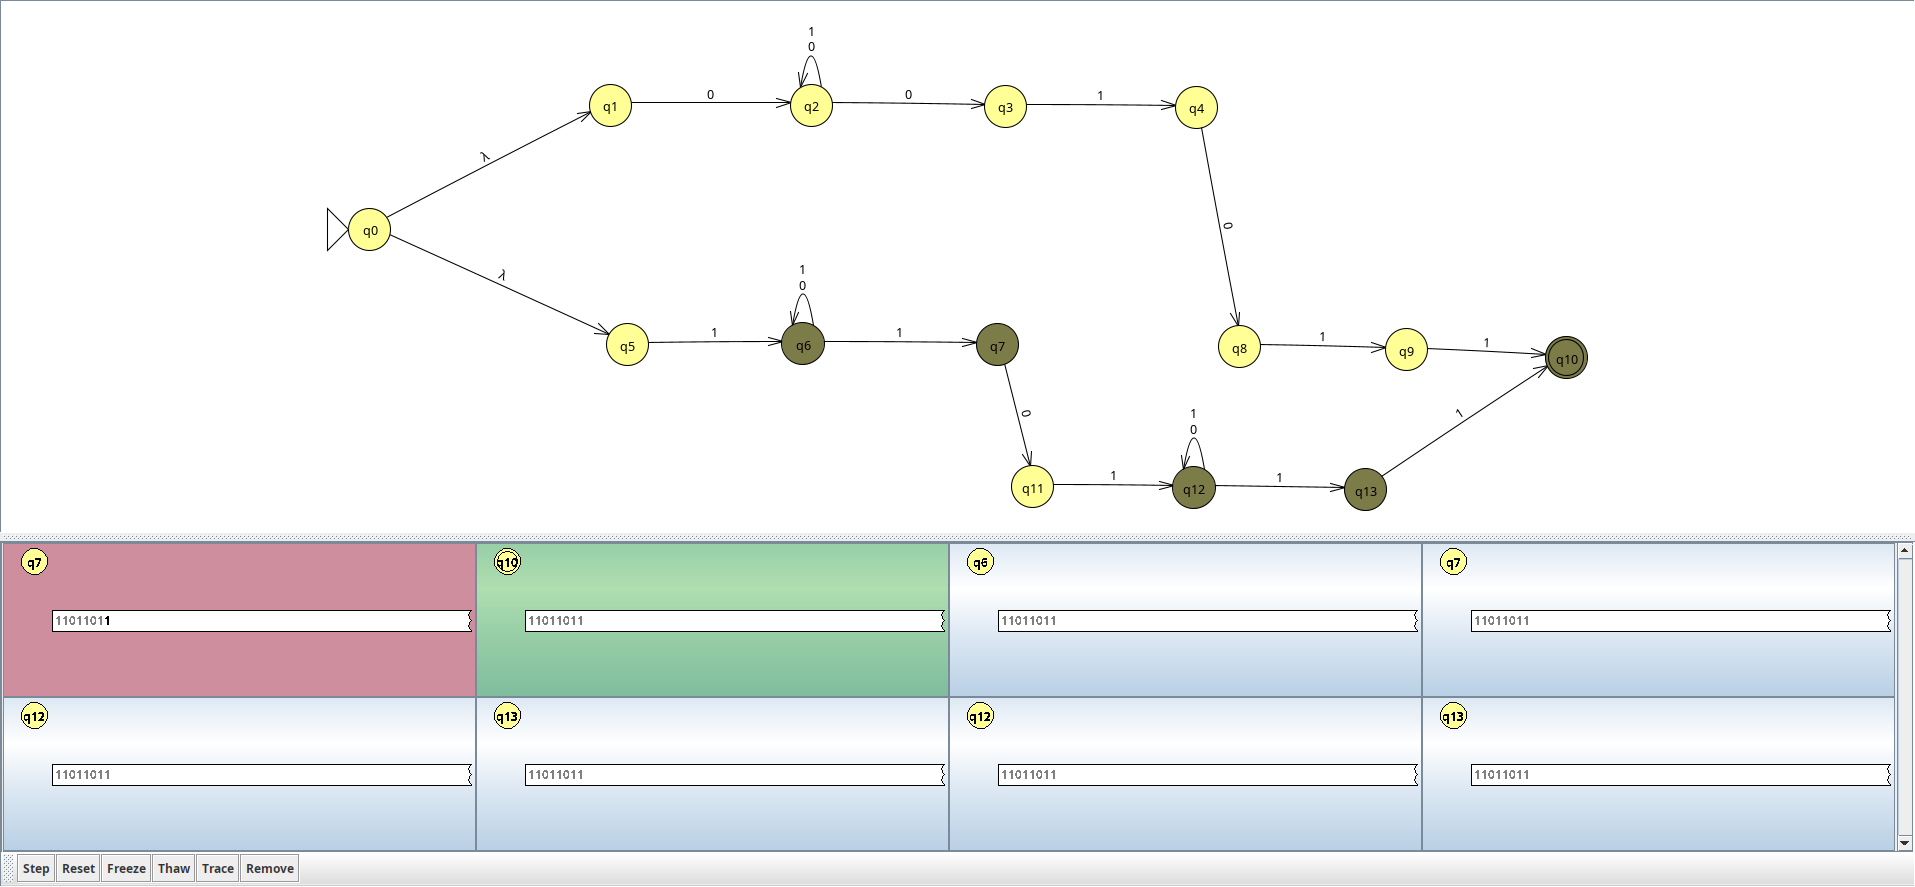
\includegraphics[width=0.85\textwidth]{../P1/img/traza_2.png}
    \caption{Procesamiento de una trama válida (Traza 2) resolviendo el no determinismo.}
    \label{fig:traza_2}
\end{figure}

\subsection{Determinización del Autómata (Transformación a AFD)}
Si bien el AFND resulta idóneo para la especificación formal del problema, su implementación directa en el microcontrolador de un dispositivo periférico es computacionalmente inviable. El hardware físico opera secuencialmente y no puede asumir la sobrecarga computacional que supone evaluar caminos de forma concurrente o realizar conjeturas sobre transiciones nulas. Se requiere, por tanto, un Autómata Finito Determinista (AFD).

Para solventar esta brecha entre abstracción y hardware, se ha aplicado el \textbf{Algoritmo de Construcción de Subconjuntos} (también conocido como algoritmo de Rabin-Scott). Mediante la función \textit{Convert to Deterministic Automaton} de JFLAP, se ha calculado el cierre-$\lambda$ de todos los estados originales. Cada nuevo estado en el AFD representa un macro-estado equivalente a un conjunto de estados del AFND original. El resultado es un autómata donde, ante un estado determinado y la lectura de un símbolo concreto, solo existe una única transición posible.

\begin{figure}[H]
    \begin{center}
        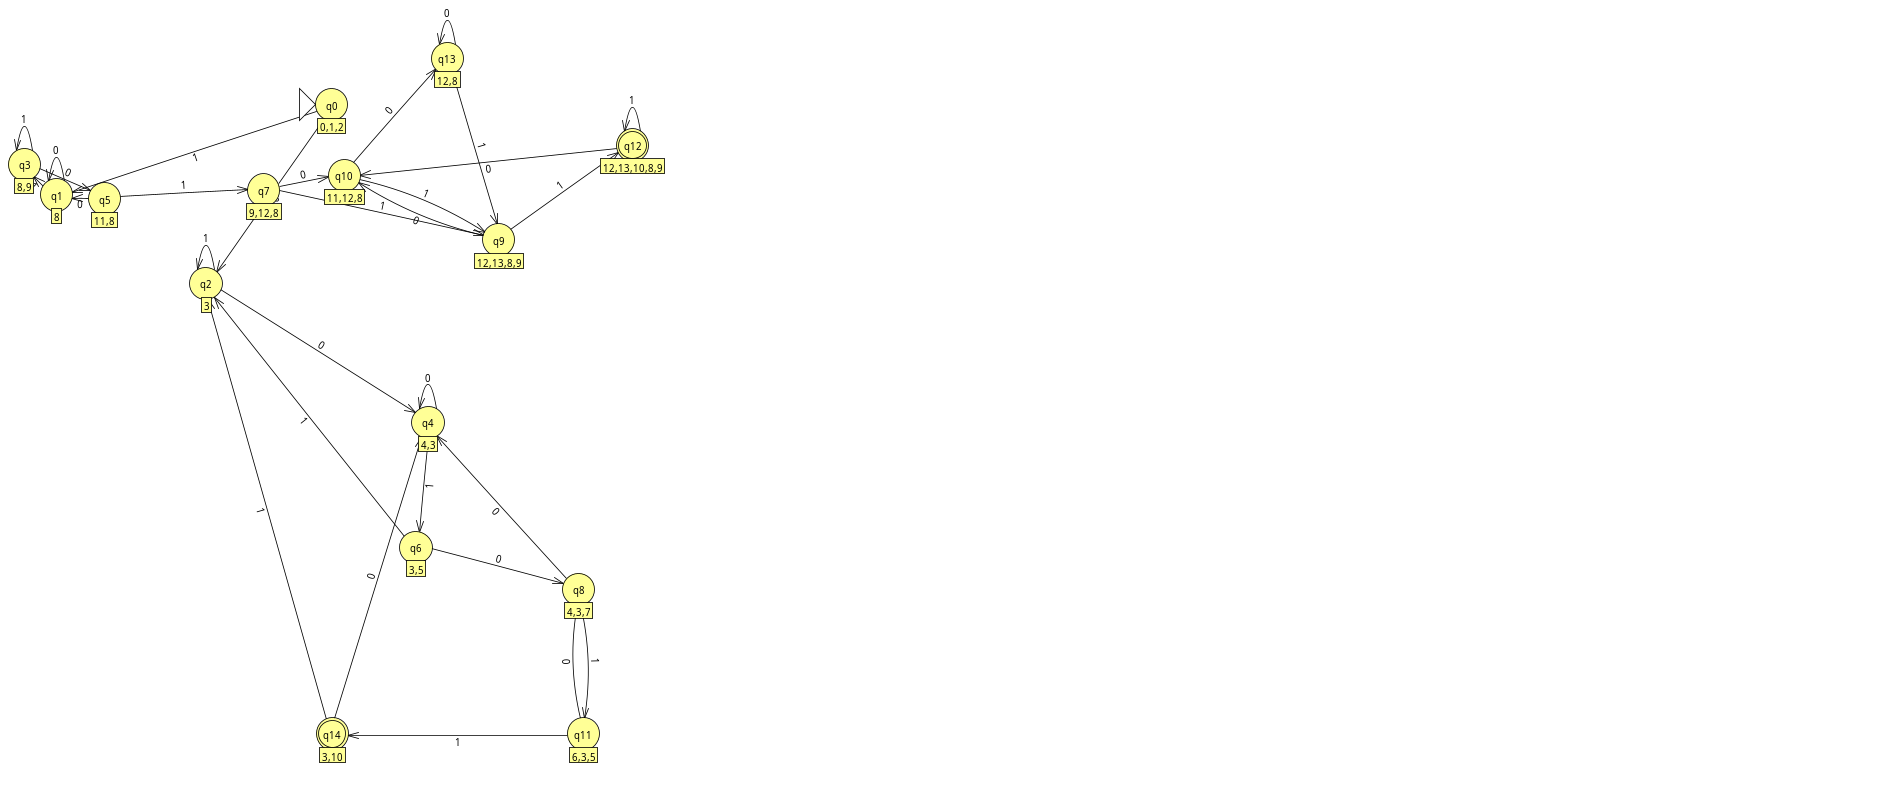
\includegraphics[width=\textwidth]{../P1/img/afd_convertido.png}
    \end{center}
    \caption{Autómata Finito Determinista (AFD) resultante de la conversión. La topología refleja un incremento de la complejidad para eliminar ambigüedades.}
    \label{fig:afd_convertido}
\end{figure}

\subsection{Optimización mediante Minimización}
El algoritmo de subconjuntos garantiza el determinismo, pero a menudo produce autómatas sobredimensionados que contienen estados redundantes o inaccesibles desde el estado inicial. En el diseño de redes, minimizar la matriz de transiciones es imperativo para reducir el uso de memoria caché y optimizar los ciclos de CPU durante el análisis de paquetes.

\bigskip

Para lograrlo, se ha recurrido al algoritmo de partición (basado en clases de equivalencia). JFLAP, mediante su herramienta \textit{Minimize DFA}, separa iterativamente los estados finales de los no finales y continúa subdividiendo estos conjuntos basándose en el comportamiento de las transiciones. Si dos o más estados derivan en las mismas respuestas ante el mismo conjunto de entradas futuras, se consideran indistinguibles y se fusionan en un único estado lógico.

\begin{figure}[H]
    \begin{center}
        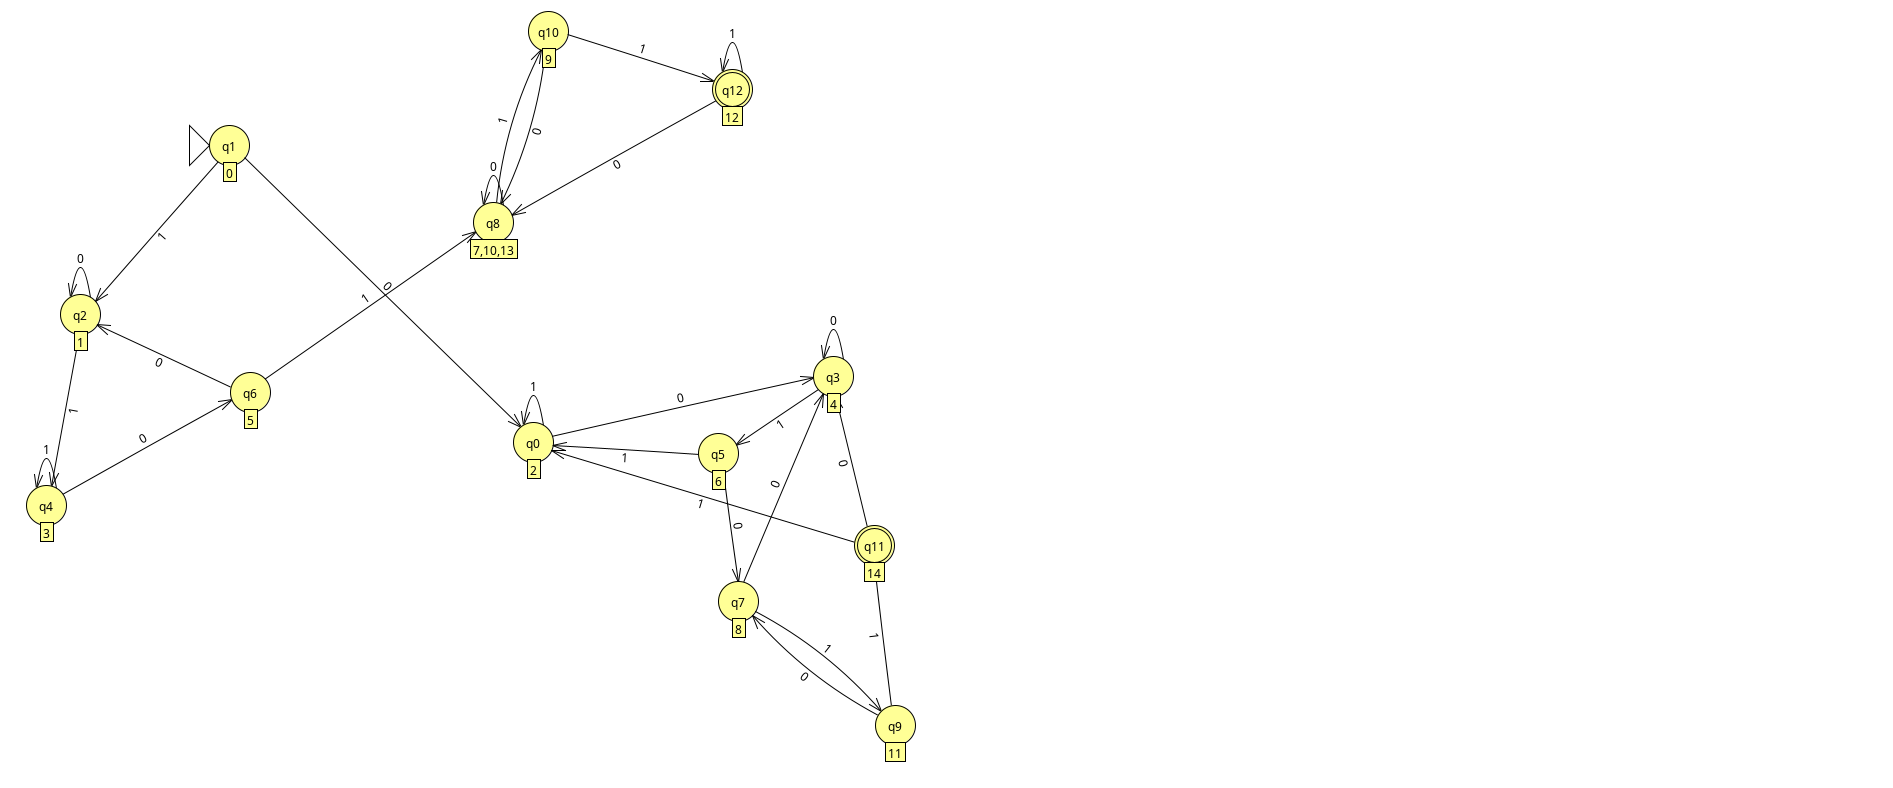
\includegraphics[width=\textwidth]{../P1/img/afd_minimo.png}
    \end{center}
    \caption{Autómata Finito Determinista Minimal. Constituye la implementación de hardware de menor coste sin alterar la capacidad de reconocimiento del lenguaje.}
    \label{fig:afd_minimo}
\end{figure}

\newpage

\subsubsection{Validación de Equivalencia del Autómata Mínimo}
Para ratificar matemáticamente que los procesos de determinización y minimización no han introducido derivas semánticas ni han alterado el lenguaje $L$ reconocido por el autómata original, se ha sometido al nuevo AFD minimal al escrutinio del banco de pruebas inicial. 

\begin{figure}[H]
    \centering
    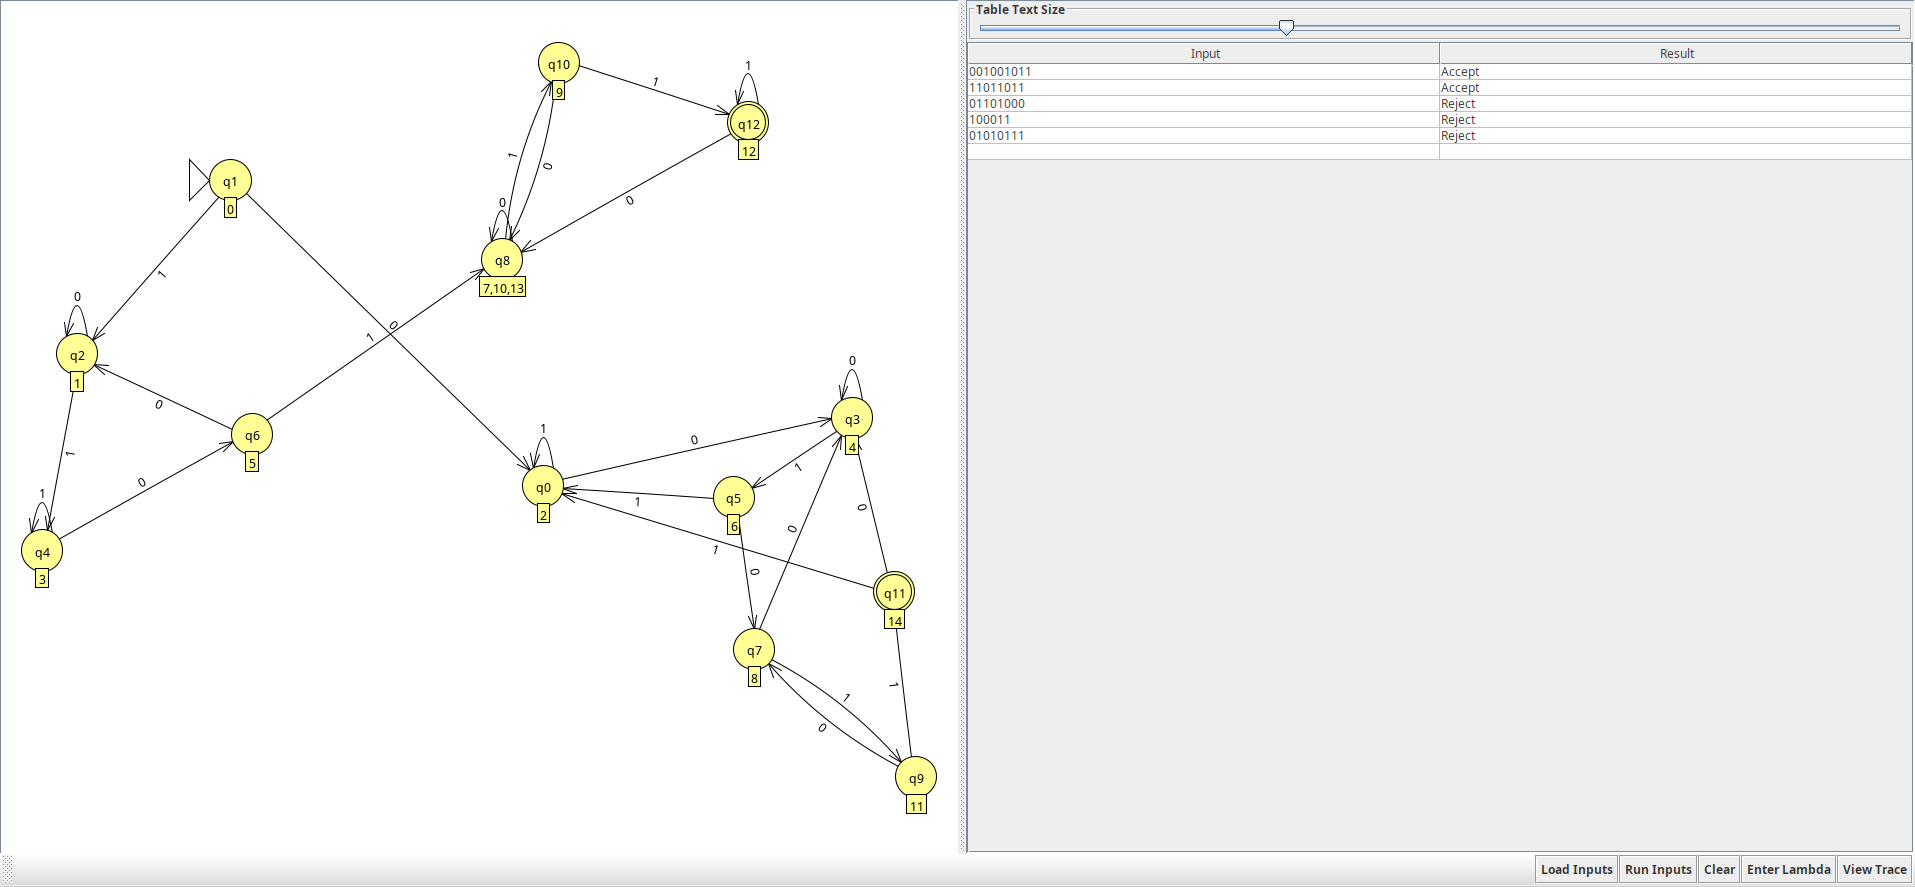
\includegraphics[width=0.85\textwidth]{../P1/img/afd_minimo_tests.png}
    \caption{Re-evaluación del banco de pruebas. El comportamiento de filtrado demuestra ser absolutamente idéntico al modelo original.}
    \label{fig:afd_minimo_tests}
\end{figure} 

\vspace{1cm}

Las trazas adjuntas a continuación corroboran que el recorrido sobre la nueva topología minimal es completamente lineal. El autómata consume un símbolo por cada transición de manera estricta y predecible, descartando paquetes erróneos inmediatamente y validando los legítimos con la máxima eficiencia.

\vspace{1cm}

\begin{figure}[H]
    \centering
    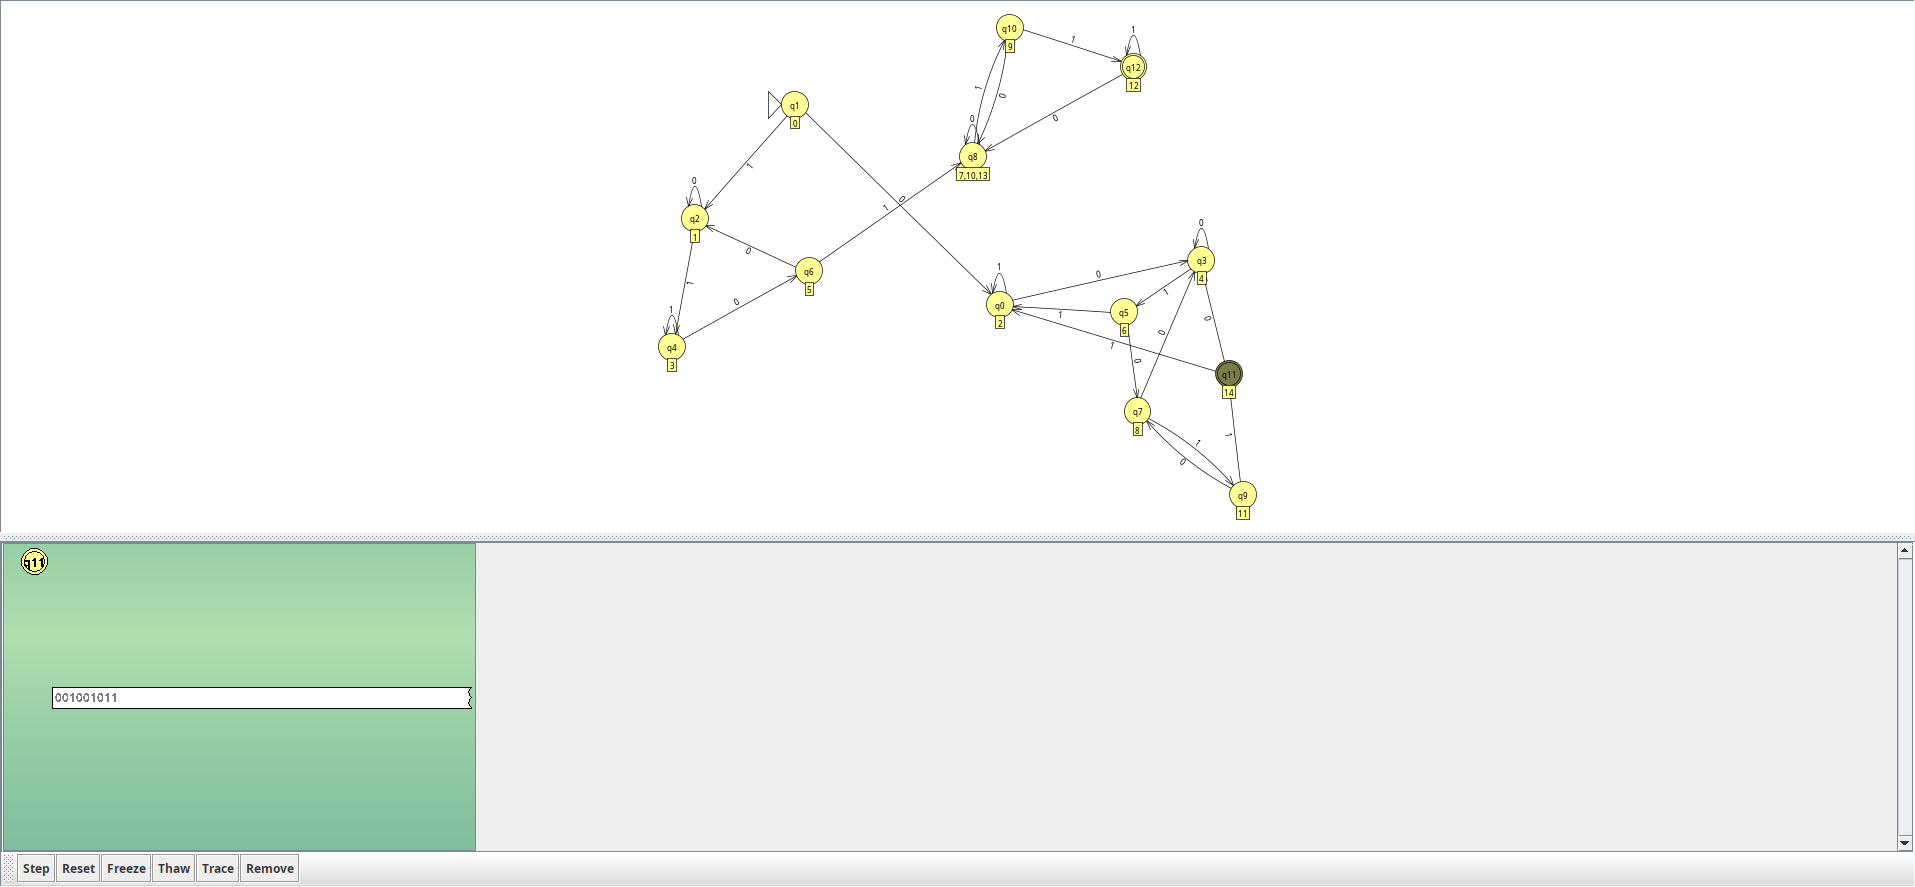
\includegraphics[width=0.85\textwidth]{../P1/img/afd_minimo_trace_1.png}
    \caption{Lectura determinista e instantánea de una trama válida (Traza 1) en la versión minimal.}
    \label{fig:afd_minimo_trace_1}
\end{figure}

\vspace{1cm}

\begin{figure}[H]
    \centering
    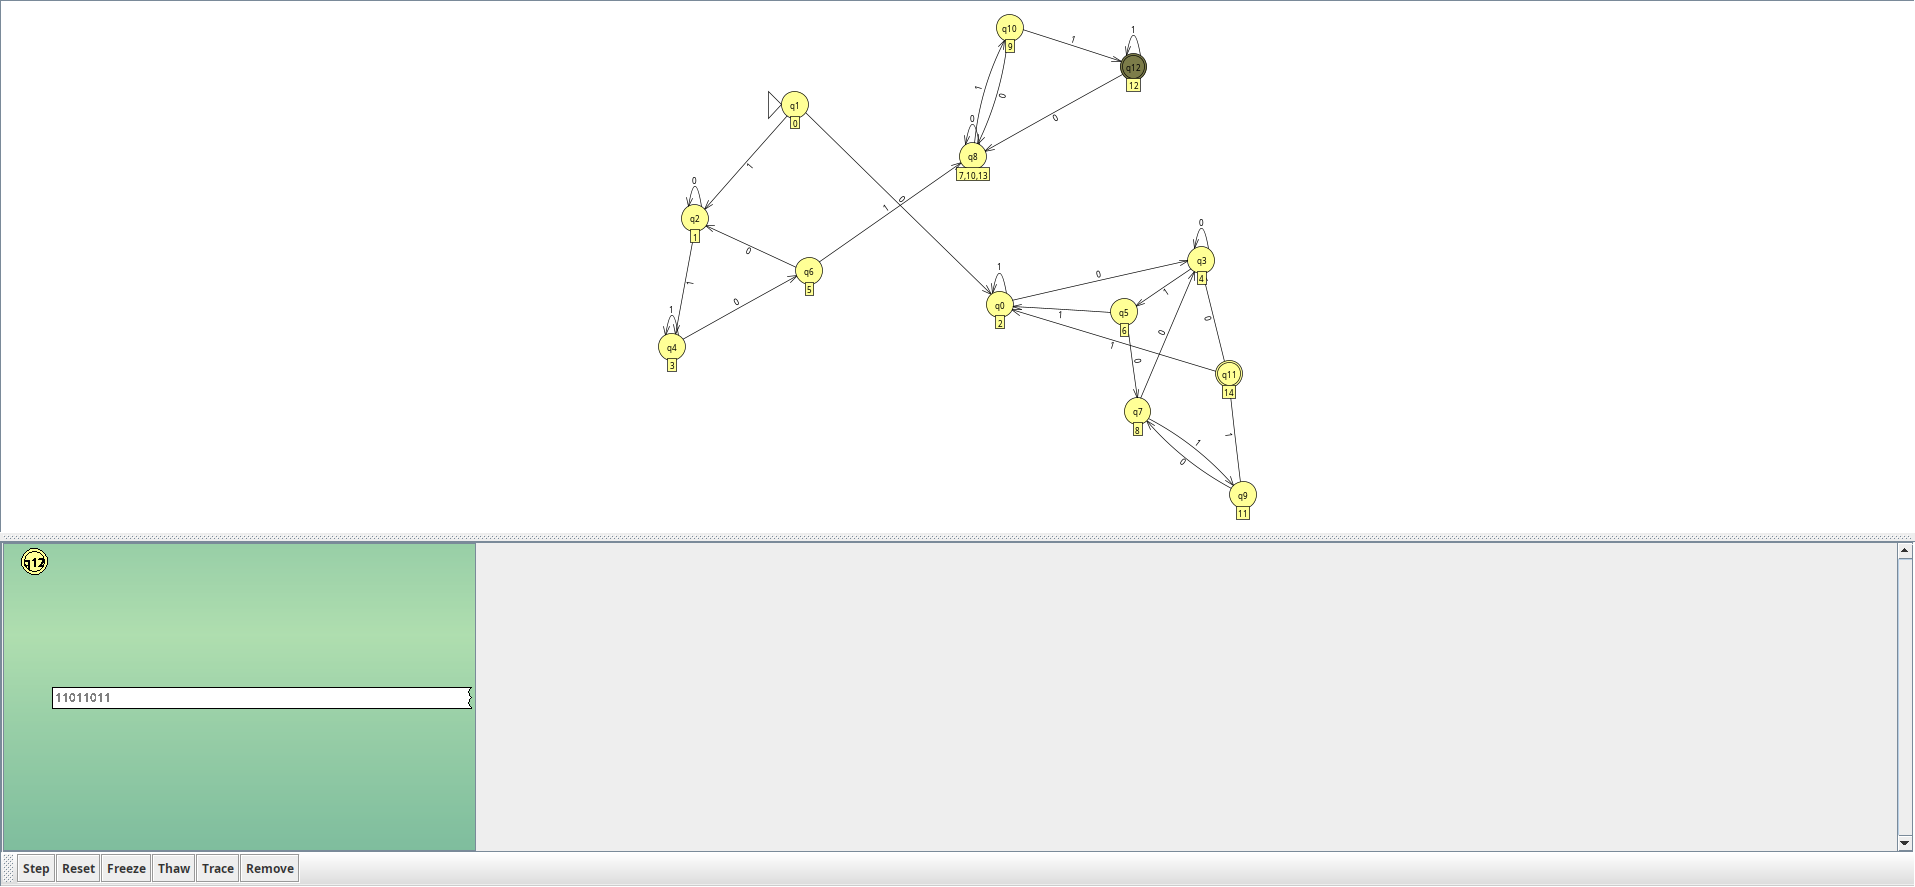
\includegraphics[width=0.85\textwidth]{../P1/img/afd_minimo_trace_2.png}
    \caption{Lectura determinista e instantánea de una trama válida (Traza 2) en la versión minimal.}
    \label{fig:afd_minimo_trace_2}
\end{figure}

\subsection{Conclusiones Finales}
El desarrollo de esta práctica demuestra la potencia y necesidad de los Modelos de Computación aplicados a la Ingeniería de Software y las Comunicaciones. Se ha completado el ciclo integral del diseño lógico:
\begin{enumerate}
    \item \textbf{Definición y Abstracción:} Partiendo de un requerimiento técnico real (telemetría de doble canal IoT), se parametrizó un lenguaje regular sujeto a estrictas validaciones de prefijo, subsecuencia y sufijo (\texttt{011}).
    \item \textbf{Modelado No Determinista:} Se diseñó un AFND apoyado en transiciones nulas para simplificar el despliegue paralelo de las reglas condicionales, confirmando su validez funcional mediante \textit{tests} automatizados.
    \item \textbf{Adaptación Tecnológica y Reducción:} Mediante procesos puramente algebraicos sustentados por el software JFLAP, el modelo fue determinizado y optimizado a su mínima expresión.
\end{enumerate}
En conclusión, el autómata final obtenido no solo reconoce de manera exacta el protocolo original, sino que presenta la forma canónica ideal para ser compilado en analizadores léxicos, expresiones regulares de firewall o grabado directamente en la lógica cableada (FPGAs) de dispositivos de red.

\newpage

\section{Práctica 2: Diseño de un Sistema de Codificación y Decodificación mediante Máquinas de Mealy}

\subsection{Introducción al Modelo Criptográfico}
El diseño de algoritmos de cifrado y descifrado en flujo continuo (\textit{stream ciphers}) es una aplicación clásica de los autómatas con salida. A diferencia de un modelo de involución pura (donde el codificador y el decodificador son topológicamente idénticos, de forma análoga al comportamiento del reflector en la máquina Enigma original), el objetivo de esta práctica es implementar un sistema asimétrico en el que la decodificación requiera una topología de autómata explícitamente diseñada para invertir la lógica de transición.

Para ello, hemos superado el modelo trivial de dos estados (basado únicamente en recordar la paridad del bit anterior) diseñando un autómata fundamentado en un \textbf{contador módulo 3}. El sistema cuenta con tres estados ($q_0, q_1, q_2$) y basa su avance cíclico exclusivamente en la lectura de bits '1'. Esta propiedad introduce una memoria acumulativa en el canal de transmisión, alterando el comportamiento frente a secuencias largas en función de la historia previa de la trama.

\subsection{Diseño del Codificador (Autómata Transductor)}
La arquitectura del codificador se ha modelado empleando una Máquina de Mealy en el entorno JFLAP. Las transiciones, expresadas en la forma entrada/salida ($a/b$), siguen la siguiente lógica de estados acumulativos:

\begin{itemize}
    \item \textbf{Estado $q_0$ (Modo Transparente):} El sistema no altera el mensaje. Transmite los bits sin inversión y permanece en $q_0$ ante la lectura de '0'. El salto al nivel superior $q_1$ se produce únicamente al procesar un '1'.
    \item \textbf{Estado $q_1$ (Inversor Nivel 1):} En este estado se invierten todas las salidas ('0' se transmite como '1'). De nuevo, el avance al estado $q_2$ está condicionado exclusivamente a la entrada de un bit '1'.
    \item \textbf{Estado $q_2$ (Inversor Nivel 2):} Similar a $q_1$, se aplican reglas de inversión. No obstante, al detectar un nuevo bit '1', el sistema completa el ciclo módulo 3, reiniciando su estado lógico de vuelta a $q_0$.
\end{itemize}

\begin{figure}[H]
    \centering
    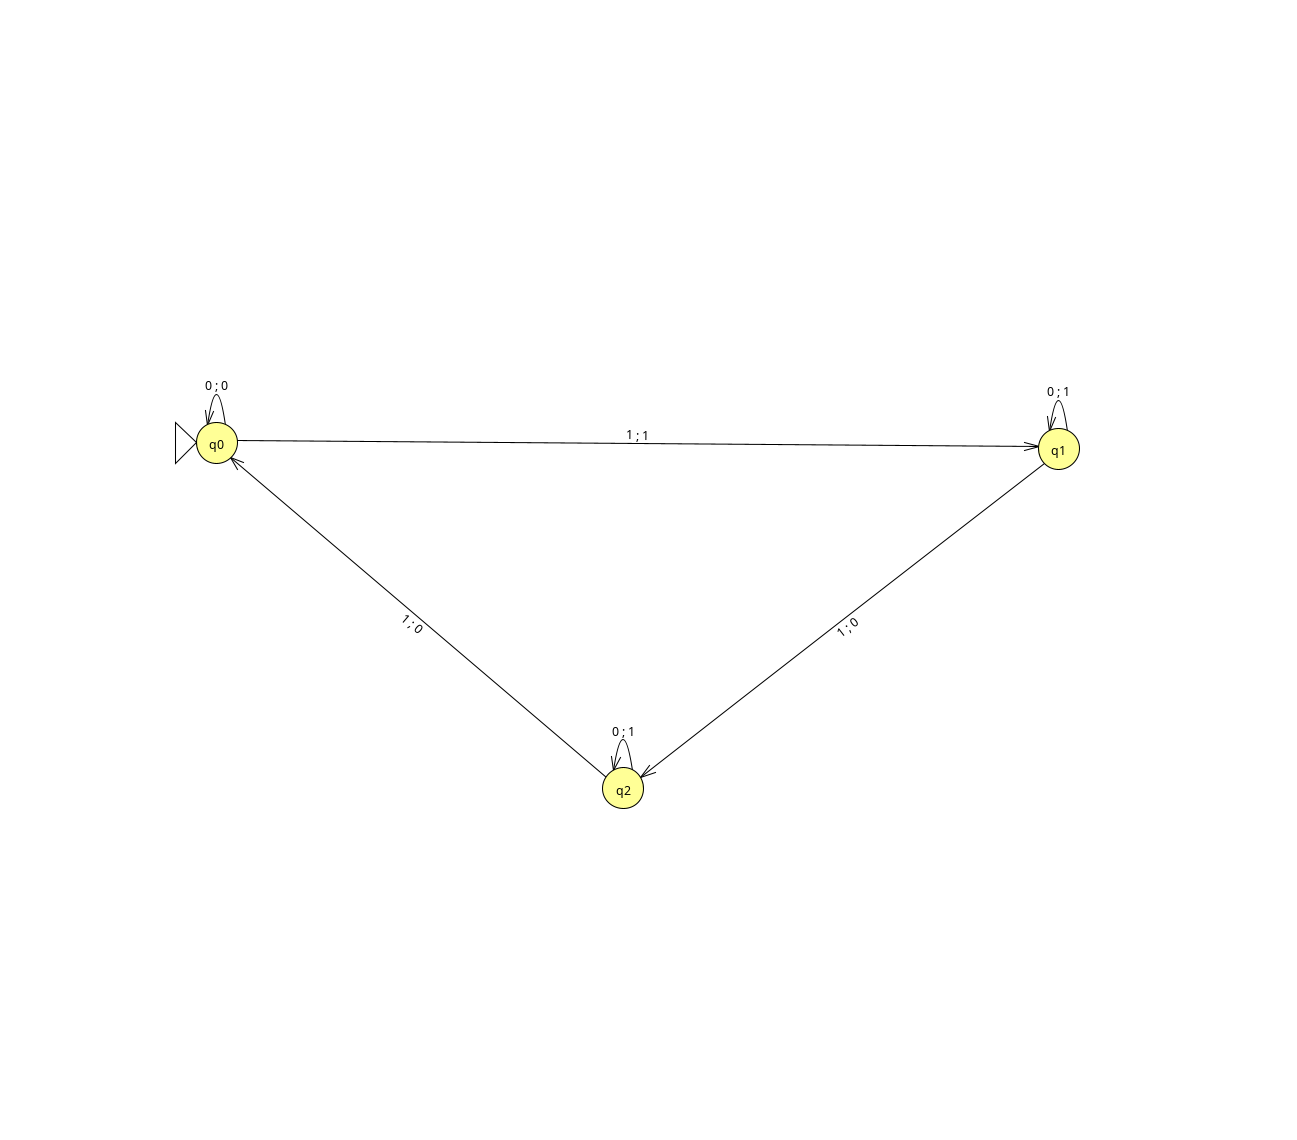
\includegraphics[width=\textwidth]{../P2/img/Codificador.png}
    \caption{Topología de la Máquina de Mealy implementando el codificador, junto con la tabla de validación de ejecución múltiple.}
    \label{fig:codificador}
\end{figure}

\subsection{Diseño del Decodificador y Propiedad Biyectiva}
Para recuperar íntegramente la información original, el módulo receptor debe simular los estados del emisor procesando el texto cifrado. Dado que el codificador alteraba su estado basándose en los bits del texto plano original, el decodificador debe inferir estos saltos a partir del texto cifrado, lo que obliga a invertir la lógica de transición cruzando los destinos. 

En la Máquina de Mealy del decodificador, observamos que las reglas de salto reconstruyen la ruta original al tiempo que las salidas deshacen las inversiones (por ejemplo, transiciones que en el emisor eran de lectura y mantenimiento, en el decodificador requieren la inversión para retornar al bit original). La topología resultante diverge de la del codificador, dotando al sistema de una robustez conceptual mayor.

\begin{figure}[H]
    \centering
    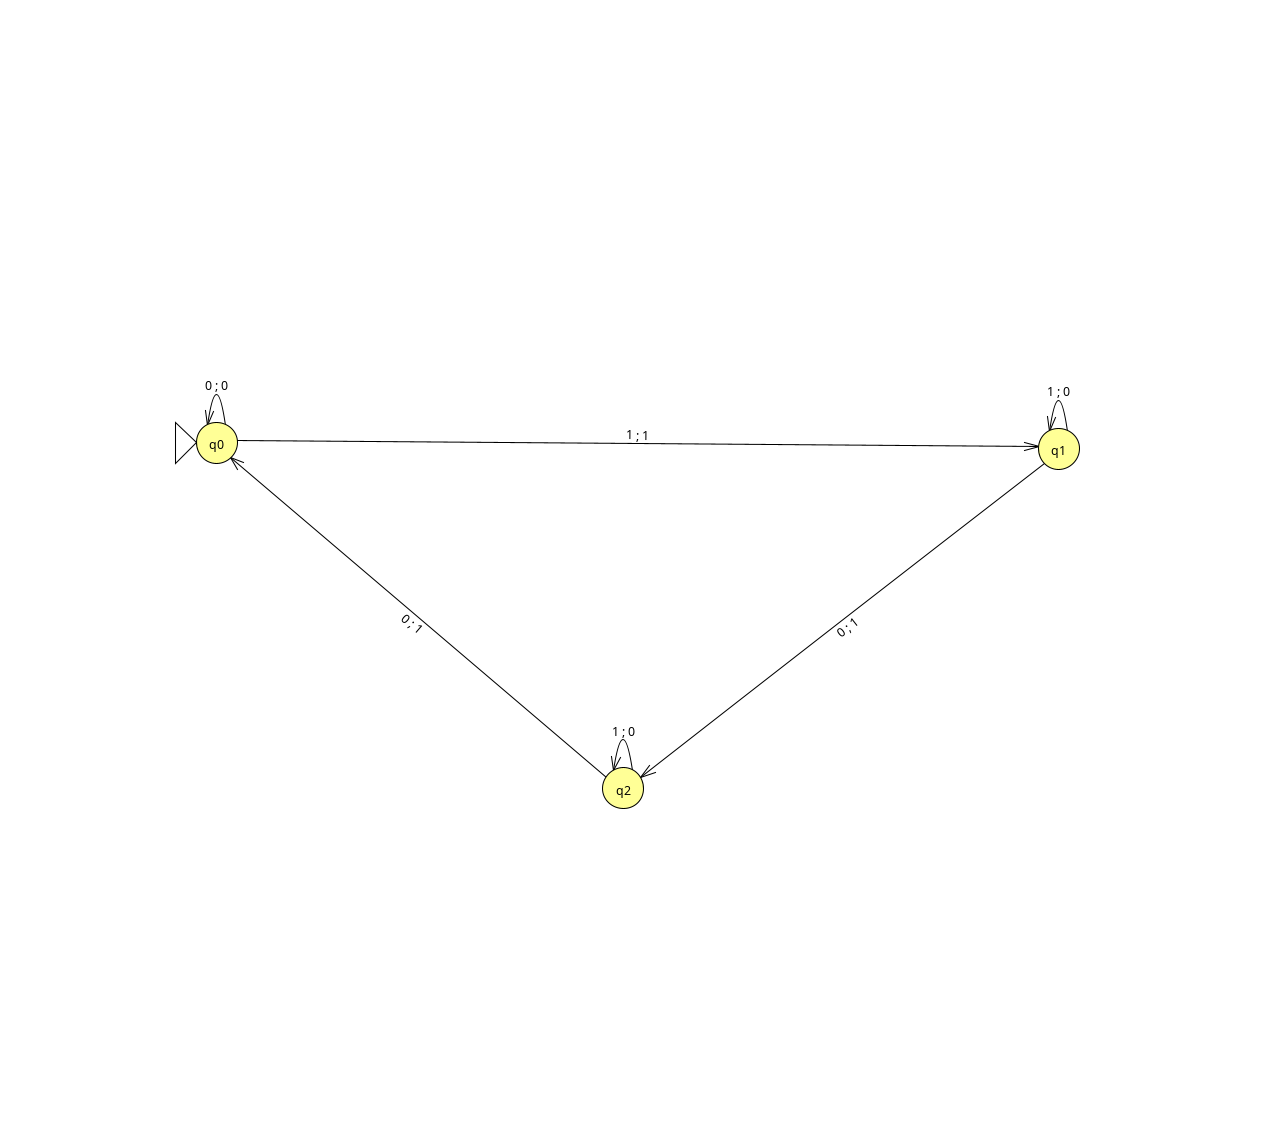
\includegraphics[width=\textwidth]{../P2/img/Decodificador.png}
    \caption{Máquina de Mealy del decodificador reconstruyendo exactamente las cadenas originales introducidas en la fase de cifrado.}
    \label{fig:decodificador}
\end{figure}

\subsection{Pruebas Empíricas y Validación Integral}
La certificación del diseño se ha verificado ejecutando las herramientas de análisis de JFLAP (\textit{Multiple Run (Transducer)}). Para evaluar el rigor del algoritmo propuesto, se seleccionaron patrones de prueba heterogéneos, incluyendo cadenas mixtas y ráfagas sostenidas de un mismo bit.

\begin{enumerate}
    \item \textbf{Prueba de Cadena Mixta (\texttt{01010}):} El codificador devuelve \texttt{01101}. Al introducir esta cadena cifrada en el decodificador, se recupera de manera exacta la secuencia \texttt{01010}.
    \item \textbf{Prueba de Ráfaga Superior (\texttt{111000}):} Las conmutaciones sucesivas provocan un ciclo completo en el autómata. El codificador computa el cifrado como \texttt{100000}. El decodificador, al leer el tercer bit, deduce el retorno a $q_0$ y restituye satisfactoriamente \texttt{111000}.
    
    \newpage
    
    \item \textbf{Prueba de Ráfaga Inferior (\texttt{000111}):} Aquí se prueba la retención del estado base antes de la alteración, arrojando el cifrado \texttt{000100}. De nuevo, el decodificador extrae exitosamente la cadena fuente \texttt{000111}.
\end{enumerate}

\begin{figure}[H]
    \centering
    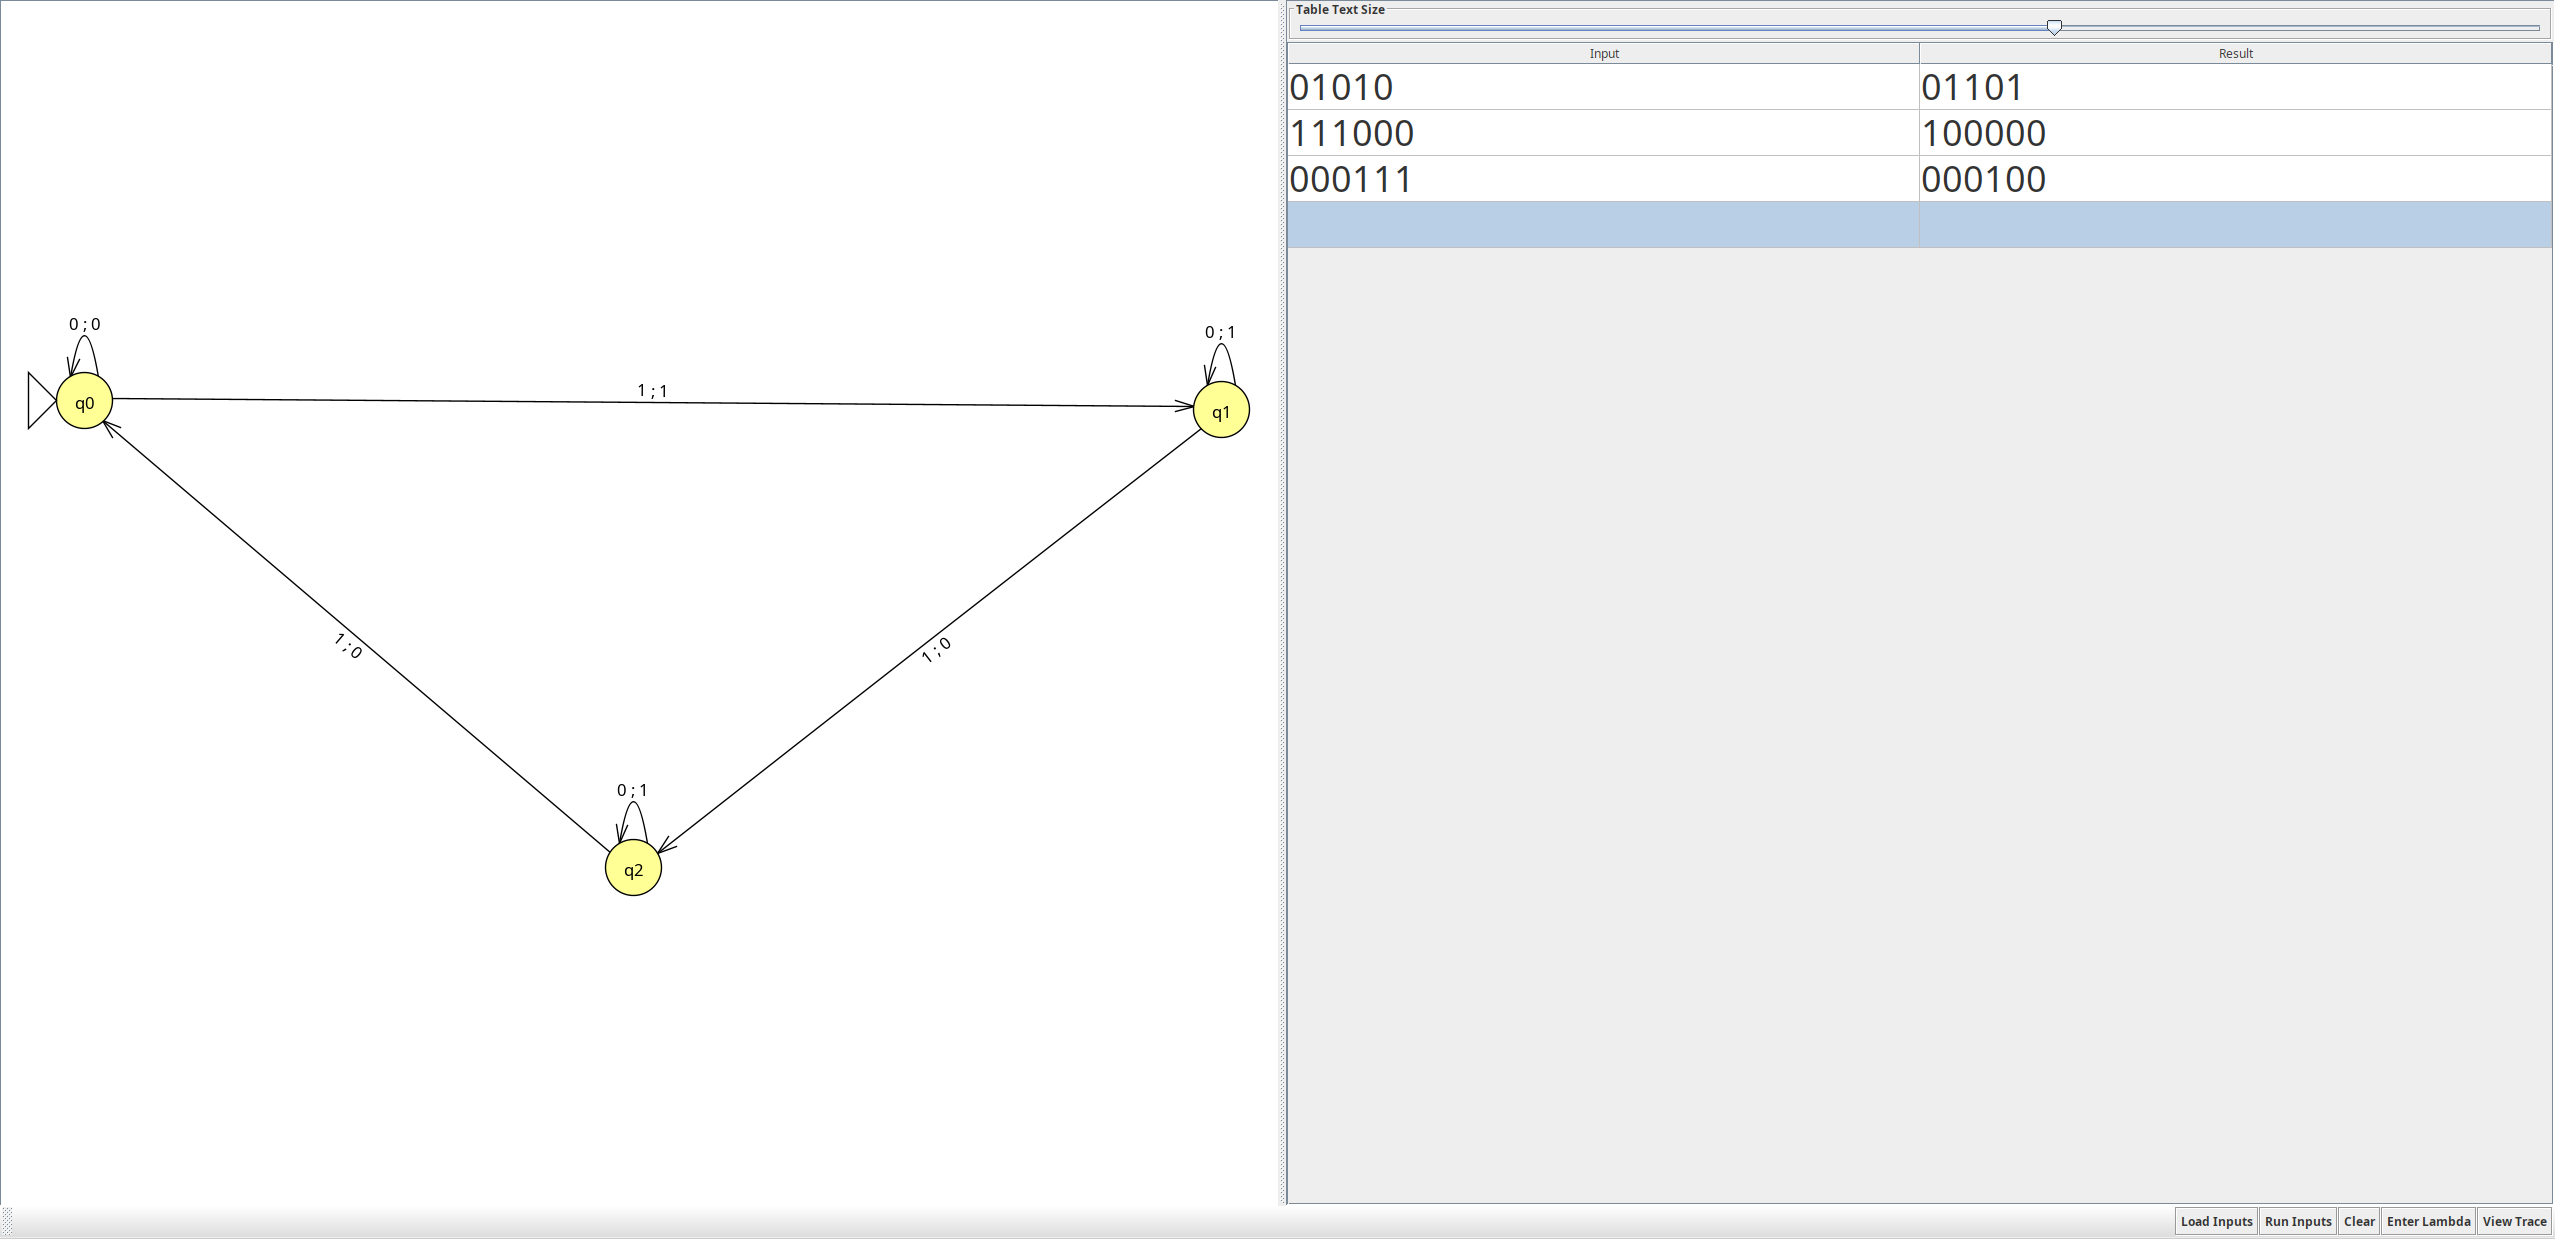
\includegraphics[width=\textwidth]{../P2/img/Codificador_Input.png}
    \caption{Ejecución múltiple del codificador verificando la transformación de las cadenas de prueba.}
    \label{fig:codificador_input}
\end{figure}

\begin{figure}[H]
    \centering
    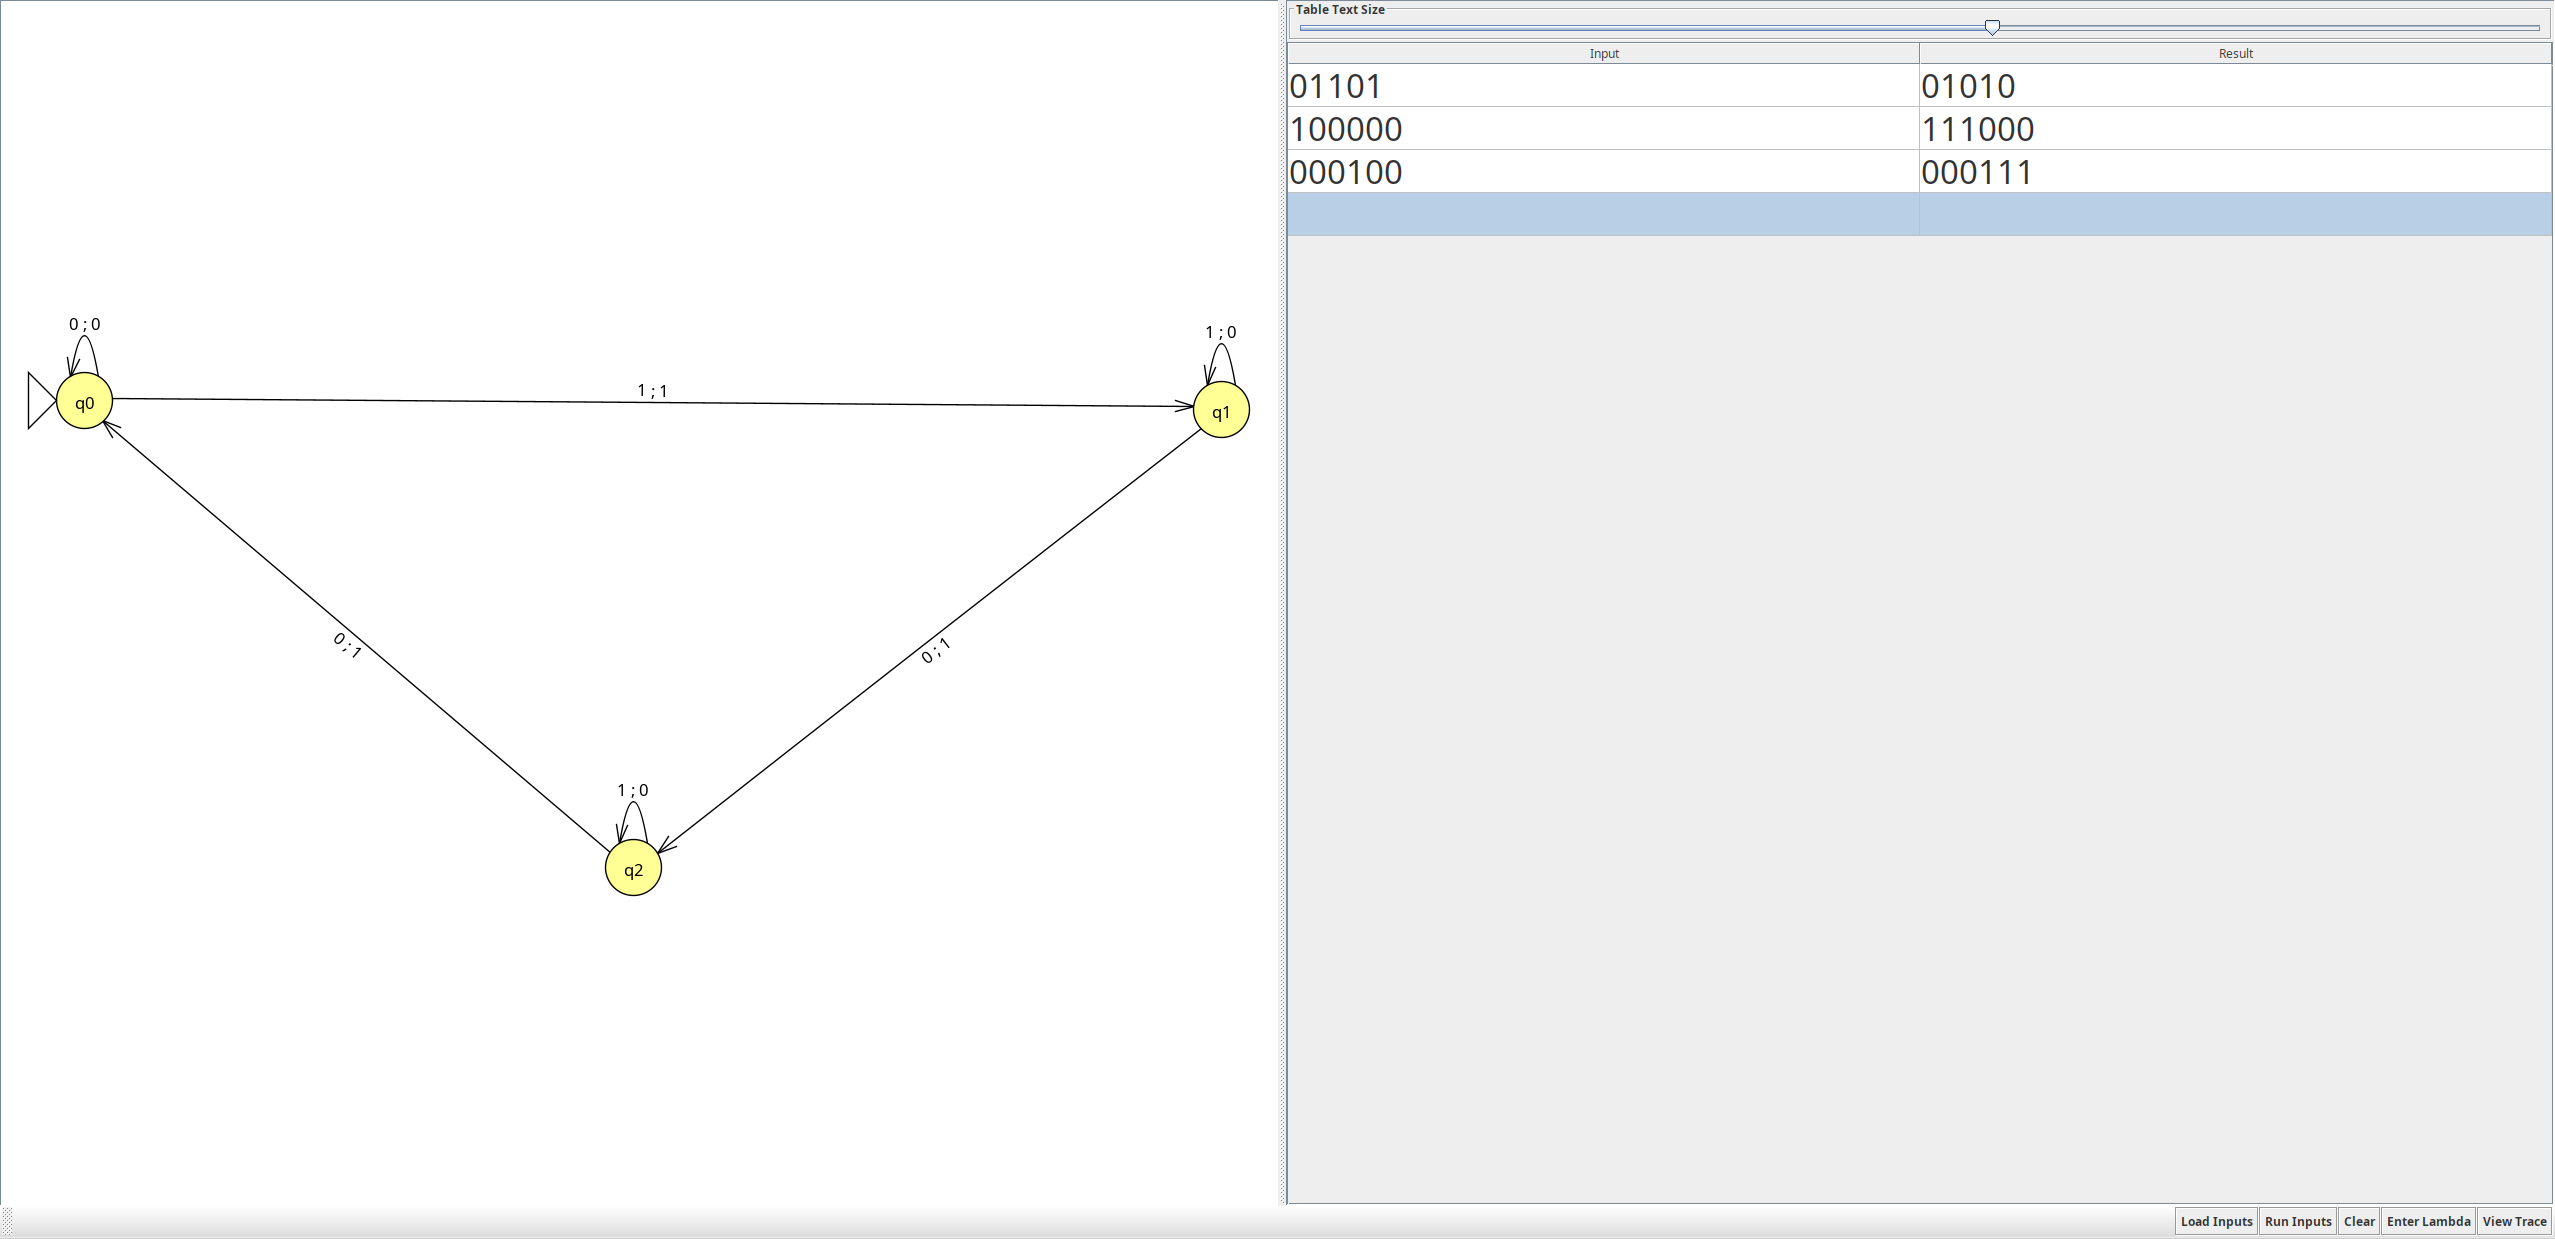
\includegraphics[width=\textwidth]{../P2/img/Decodificador_Input.png}
    \caption{Ejecución múltiple del decodificador demostrando la recuperación exacta y biyectiva de los mensajes originales.}
    \label{fig:decodificador_input}
\end{figure}

Estos resultados empíricos validan la total biyectividad matemática entre los autómatas. El diseño cumple su objetivo demostrando que el estado interno del flujo de cifrado permite transmisiones asimétricas sin pérdida ni corrupción del paquete de datos.

\subsection{Conclusiones Finales}
El desarrollo de esta segunda práctica ha evidenciado la versatilidad de las Máquinas de Mealy (autómatas con salida) para el diseño de sistemas criptográficos de flujo continuo. El trabajo realizado nos permite concluir lo siguiente:
\begin{enumerate}
    \item \textbf{Gestión de Memoria con Estados:} Se superaron los cifradores básicos mediante la implementación de un contador módulo 3 condicionado. Esto demostró cómo el autómata puede "recordar" el histórico de la trama (los bits '1' leídos) para alterar su comportamiento de forma dinámica a lo largo de secuencias extensas.
    \item \textbf{Diseño Asimétrico Integral:} Se logró construir un modelo donde el decodificador no es un mero espejo topológico del emisor, sino un transductor invertido lógicamente, capaz de inferir los saltos de estado basándose exclusivamente en el texto cifrado.
    \item \textbf{Robustez Matemática:} Las pruebas empíricas mediante \textit{Multiple Run} confirmaron empíricamente la propiedad biyectiva del sistema diseñado. Quedó garantizado que cualquier secuencia introducida es recuperable sin pérdida de información, falsos positivos ni desincronización de estados.
\end{enumerate}
En síntesis, este modelo reafirma que los autómatas finitos transductores representan una base algorítmica óptima y altamente eficiente para la implementación en hardware de sistemas de codificación y decodificación en las comunicaciones digitales.

\newpage

% =======================================================
%                    PRÁCTICA 3
% =======================================================
\section{Práctica 3: Construcción de un Analizador Léxico con Flex para \mbox{Generación} de Gráficos SVG}

\subsection{Introducción al Lenguaje de Tortuga}
En esta tercera práctica se ha abordado la fase léxica del desarrollo de procesadores de lenguajes mediante el uso de la herramienta \textbf{Flex}. El objetivo central ha sido construir un escáner capaz de procesar un Lenguaje de Dominio Específico (DSL) basado en la clásica geometría de la ``Tortuga'' (inspirado en el lenguaje Logo) e interpretar sus comandos para traducirlos, de forma directa, a un archivo de gráficos vectoriales escalables (SVG).

El conjunto de instrucciones a evaluar incluye acciones de traslación (\texttt{AVANZA}), rotación (\texttt{GIRA}), control de trazado (\texttt{SUBE}, \texttt{BAJA}), ajustes estilísticos (\texttt{COLOR}) y estructuras iterativas básicas sin anidamiento (\texttt{REPITE}).

\subsection{Diseño del Analizador Léxico (Patrones y Estados)}
Bajo el principio fundamental de diseño léxico que dicta que \textit{``las reglas reconocen, las acciones calculan''}, la estructura del archivo Flex (\texttt{tortuga.l}) se ha dividido de manera que la carga del emparejamiento semántico recae sobre las Expresiones Regulares, mientras que el cálculo trigonométrico y el ensamblado del archivo XML (SVG) se delega a las funciones incrustadas en código C.

\subsubsection{Gestión de Iteraciones mediante Condiciones de Arranque}
Para resolver la problemática del comando \texttt{REPITE}, se ha hecho un uso avanzado de las \textbf{condiciones de arranque} proporcionadas por Flex. Dado que el flujo interno del escáner está diseñado para consumir caracteres de manera secuencial hacia adelante, este no posee la capacidad nativa de retroceder el puntero de lectura para volver a evaluar un bloque de código iterativo.

Para sortear esta limitación computacional, se ha implementado un estado exclusivo denotado como \texttt{\%x BUCLE}. Cuando el escáner identifica la firma de apertura de un ciclo (\texttt{REPITE [N] [}), transiciona desde su estado inicial hacia este estado aislado. Durante la fase de bucle, las reglas regulares no ejecutan acciones de dibujado inmediato; en su lugar, actúan como recolectoras, almacenando los tokens reconocidos junto con sus argumentos en un array de estructuras internas. Al detectar el carácter de cierre (\texttt{]}), el autómata retorna a la condición inicial y dispara un ciclo en C que ejecuta los comandos guardados el número de veces estipulado.

\subsubsection{Definición de Expresiones Regulares Clave}
Para garantizar la captura robusta de los comandos, se han empleado diversas estrategias en la sección de reglas formales:
\begin{itemize}
    \item \textbf{Flexibilidad de Casos:} Se ha invocado la directiva \texttt{\%option case-insensitive} para asegurar que comandos como \texttt{AVANZA}, \texttt{Avanza} o \texttt{avanza} sean reconocidos por el mismo patrón abstracto.
    \item \textbf{Filtrado de Argumentos:} Se ha definido una macro estandarizada \texttt{NUM -?[0-9]+} para interceptar tanto longitudes de trazado positivas como ángulos de giro negativos.
    \item \textbf{Cajones de Sastre:} Se han implementado dos reglas escoba mediante el prefijo de comodín \texttt{<*>}. La primera descarta silenciosamente blancos y tabulaciones, garantizando que no generen interferencias gráficas. La segunda captura secuencias de caracteres no reconocidos, deteniéndose ante cualquier error léxico (como un comando mal escrito) e imprimiendo la advertencia correspondiente mediante el registro de línea mantenido automáticamente por \texttt{yylineno}.
\end{itemize}

\subsection{Lógica de Acciones y Ensamblado de Salida en C}
La carga semántica del proyecto radica en el bloque principal en C incluido dentro del fichero Flex.

\begin{enumerate}
    \item \textbf{Estado de la Tortuga:} Se han declarado variables globales que actúan como la memoria posicional del puntero de dibujo: coordenadas euclidianas ($x$, $y$), la inclinación actual (\texttt{angulo}), el color del trazo (\texttt{color}) y una bandera lógica (\texttt{lapiz}) que determina si los movimientos generan huella vectorial.
    \item \textbf{Cálculo Trigonométrico:} Al procesar el comando \texttt{AVANZA d}, la función en C efectúa un cambio de base transformando el avance lineal en incrementos cartesianos, aplicando las fórmulas trigonométricas $x_{nueva} = x + d \cdot \cos(\theta)$ y $y_{nueva} = y + d \cdot \sin(\theta)$, con el ángulo $\theta$ previamente convertido a radianes.
    \item \textbf{Generación del Archivo Vectorial:} Cada avance con el lápiz activo genera en memoria una etiqueta \texttt{<line>} propia del estándar SVG. En paralelo, se evalúan constantemente los máximos y mínimos dimensionales para computar, al término de la lectura del fichero, los atributos correctos de encuadre en la directiva \texttt{viewBox}.
\end{enumerate}

\subsection{Automatización del Entorno (Makefile)}
En entornos UNIX, el flujo de procesamiento léxico involucra varios eslabones de compilación (desde la especificación \texttt{.l} hasta el binario ejecutable final). Para orquestar esto de forma transparente y facilitar la labor de evaluación por parte del profesorado, se ha diseñado un \texttt{Makefile} estructurado con reglas explícitas que automatiza tanto la compilación como la ejecución de las pruebas.

\subsubsection{Estructura de Directorios}
Para una correcta evaluación, el proyecto se entrega estructurado de forma modular dentro de la carpeta \texttt{P3}. La disposición inicial de los ficheros en el archivo comprimido ZIP es la siguiente:
\begin{itemize}
    \item \textbf{\texttt{src/}:} Contiene el código fuente original de Flex (\texttt{tortuga.l}).
    \item \textbf{\texttt{pruebas/}:} Almacena los archivos de texto con los comandos de prueba (\texttt{poligono.txt} y \texttt{errores.txt}).
    \item \textbf{\texttt{Makefile}:} Archivo de orquestación ubicado en la raíz de la carpeta \texttt{P3}.
\end{itemize}
\newpage
\textbf{Nota sobre la generación de carpetas:} Las carpetas de salida (\texttt{img/} para los gráficos SVG y \texttt{bin/} para los ejecutables) se omiten intencionadamente en la entrega. El propio \texttt{Makefile} incluye una directiva preparatoria que se encarga de crear estos directorios automáticamente en el equipo del evaluador antes de realizar la compilación, manteniendo un entorno limpio.

A continuación se detalla el código del \texttt{Makefile} utilizado en el proyecto:

\begin{verbatim}
# Definición de variables
FLEX = flex
CC = gcc
CFLAGS = -lm

# Carpetas
SRC_DIR = src
BIN_DIR = bin
TEST_IN_DIR = pruebas
TEST_OUT_DIR = img

# Archivos
LEX_FILE = $(SRC_DIR)/tortuga.l
C_FILE = $(SRC_DIR)/lex.yy.c
EXEC = $(BIN_DIR)/tortuga

# Archivos de prueba
TEST1_IN = $(TEST_IN_DIR)/poligono.txt
TEST1_OUT = $(TEST_OUT_DIR)/poligono.svg
TEST2_IN = $(TEST_IN_DIR)/errores.txt
TEST2_OUT = $(TEST_OUT_DIR)/errores.svg

# Regla por defecto: compilar y ejecutar todo
all: prepare $(EXEC) run

# Crear directorios si no existen (separados línea a línea para evitar fusiones)
prepare:
	@mkdir -p $(BIN_DIR)
	@mkdir -p $(SRC_DIR)
	@mkdir -p $(TEST_IN_DIR)
	@mkdir -p $(TEST_OUT_DIR)

# Regla para compilar el ejecutable
$(EXEC): $(C_FILE)
	@echo "Compilando el ejecutable de C..."
	$(CC) $(C_FILE) -o $(EXEC) $(CFLAGS)

# Regla para generar el .c con flex
$(C_FILE): $(LEX_FILE)
	@echo "Ejecutando Flex..."
	$(FLEX) -o $(C_FILE)    $(LEX_FILE)

# Regla para ejecutar las pruebas
run: $(EXEC)
	@echo "Ejecutando pruebas..."
	@if [ -f "$(TEST1_IN)" ]; then \
		./$(EXEC) "$(TEST1_IN)" > "$(TEST1_OUT)"; \
		echo " -> $(TEST1_OUT) generado."; \
	else \
		echo "Aviso: No se encontró $(TEST1_IN)"; \
	fi
	@if [ -f "$(TEST2_IN)" ]; then \
		./$(EXEC) "$(TEST2_IN)" > "$(TEST2_OUT)"; \
		echo " -> $(TEST2_OUT) generado."; \
	else \
		echo "Aviso: No se encontró $(TEST2_IN)"; \
	fi

# Limpiar archivos generados y BORRAR carpetas bin e img
clean:
	@echo "Limpiando archivos y carpetas generadas..."
	rm -f $(C_FILE)
	rm -rf $(BIN_DIR)
	rm -rf $(TEST_OUT_DIR)

# Declarar que clean, prepare, run, all no son archivos
.PHONY: all prepare clean run
\end{verbatim}

\subsubsection{Explicación de las directivas de compilación}
Para compilar y testear el proyecto, únicamente es necesario abrir una terminal en la raíz y ejecutar comandos básicos de \texttt{make}. La lógica de dependencias está diseñada para agilizar el flujo de trabajo:
\begin{itemize}
    \item \textbf{\texttt{make} o \texttt{make all}:} Es la regla por defecto. Asegura la estructura de directorios (\texttt{prepare}), invoca a Flex para traducir el código léxico, lo compila con GCC enlazando estáticamente la librería matemática (\texttt{-lm}) y finalmente ejecuta las simulaciones sobre los archivos de prueba para escupir automáticamente los SVG (\texttt{run}).
    \item \textbf{\texttt{make clean}:} Elimina los artefactos autogenerados (como \texttt{lex.yy.c}) y borra por completo las carpetas de salida (\texttt{bin/} e \texttt{img/}), devolviendo el directorio a su estado de desarrollo inicial perfecto para ser comprimido y entregado.
    \item \textbf{Gestión de dependencias temporales:} Las reglas \texttt{\$(EXEC)} y \texttt{\$(C\_FILE)} observan los cambios en el código. Si se modifica \texttt{tortuga.l}, el \texttt{Makefile} reconstruye todo el árbol. Esto ahorra valiosos ciclos de compilación.
\end{itemize}

\newpage
\subsection{Verificación Empírica y Casos de Prueba}

El sistema resultante se ha sometido a validación mediante dos flujos de texto preestablecidos.

\subsubsection{Caso 1: Trazado de Geometría Regular}
Se sometió el analizador al documento de entrada \texttt{poligono.txt}, cuyo código invoca la construcción iterada de un polígono de seis lados mediante el comando repetitivo.

\begin{verbatim}
COLOR azul
BAJA
REPITE 6 [
  AVANZA 60
  GIRA 60
]
SUBE
\end{verbatim}

La salida de la compilación originó satisfactoriamente el archivo \texttt{poligono.svg}, logrando empaquetar de forma transparente las coordenadas trigonométricas necesarias para renderizar la figura descrita.

\begin{figure}[H]
    \centering
    \includegraphics[width=0.45\textwidth]{../P3/img/poligono.png}
    \caption{Resultado visual del archivo SVG generado tras la evaluación del primer lote de prueba, demostrando un procesamiento matemático correcto de los bucles léxicos.}
    \label{fig:prueba1}
\end{figure}

\newpage

\subsubsection{Caso 2: Tolerancia y Gestión de Errores}
El segundo bloque de validación, \texttt{errores.txt}, fue inyectado con el propósito explícito de comprobar la solidez del autómata frente a comportamientos indebidos:

\begin{verbatim}
COLOR      rojo
BAJA
REPITE 4   [
  AVANZA 50
  TELETRANSPORTA 100
  REPITE 2 [
    GIRA 45
  ]
]
    EXPLOTA 99
\end{verbatim}

Ante esta entrada, el sistema se comportó de manera estrictamente robusta. En primer lugar, los identificadores anómalos (\texttt{TELETRANSPORTA} y \texttt{EXPLOTA}) fueron correctamente redirigidos hacia el cajón de sastre de error, alertando al usuario en la salida estándar de errores (stderr) con la línea exacta de la infracción. En segundo lugar, al intentar anidar un bucle de repetición dentro de otro, el autómata activó la validación estática incorporada en su estado \texttt{BUCLE}, impidiendo el cómputo y emitiendo un mensaje de rechazo de sintaxis sin corromper el fichero de salida vectorial hasta el momento de la interrupción.

\begin{figure}[H]
    \centering
    \includegraphics[width=0.45\textwidth]{../P3/img/errores.png}
    \caption{Captura del trazo interrumpido renderizado en \texttt{errores.svg}. Se evidencia que el escáner dibuja todo el código legítimo antes de interceptar el intento de anidamiento ilegal.}
    \label{fig:prueba2}
\end{figure}

\newpage

\subsection{Conclusiones Finales}
Esta tercera práctica ha consolidado los conceptos algorítmicos teóricos relativos a las máquinas de estado mediante una aplicación práctica directa de análisis de secuencias. Se ha puesto de manifiesto que los lenguajes regulares, aunque poseen limitaciones matemáticas demostradas en su jerarquía (como la incapacidad estructural para contar balanceo de anidamientos), pueden ser dotados de cierta persistencia temporal en memoria mediante el uso de estados exclusivos en la herramienta \textbf{Flex}. Esta sinergia entre el reconocimiento algorítmico rápido de patrones en el archivo \texttt{.l} y la computación lógica delegada al código empotrado en C, ha permitido construir un motor gráfico de procesamiento integral robusto y plenamente operativo.

\newpage

% =======================================================
%                    SECCIÓN 4
% =======================================================
\section{Valoración Global y Perspectivas Profesionales}

A lo largo de este cuatrimestre, el desarrollo de estas prácticas nos ha permitido aterrizar conceptos que, en las primeras clases, parecían pura teoría matemática. Pasar de los esquemas en la pizarra a diseñar la lógica directamente mediante software ha sido clave para entender realmente qué ocurre ``bajo el capó'' de los sistemas que utilizamos a diario. 

Durante las dos primeras prácticas, vimos de forma muy visual con JFLAP que los autómatas y las máquinas de Mealy no son simples grafos, sino el núcleo lógico que hay detrás de un protocolo de red o de un sistema básico de cifrado. Sin embargo, ha sido con la tercera práctica donde hemos notado el salto definitivo hacia la programación real. Utilizar Flex nos ha obligado a unir la potencia de las expresiones regulares con código C puro, enseñándonos que el autómata es el que reconoce el texto, pero es nuestra lógica la que realmente trabaja con él.

Siendo realistas, es muy poco probable que en nuestro futuro puesto de trabajo nos pidan dibujar un autómata finito a mano o diseñar una máquina de Mealy desde cero para hacer una aplicación web. Sin embargo, la forma de pensar que hemos entrenado aquí tiene una aplicación directa y muy demandada en la empresa actual:

\begin{itemize}
    \item \textbf{Procesamiento de datos y Expresiones Regulares:} En sectores como la Ciberseguridad, el Big Data o el trabajo de sistemas (DevOps), lidiar con gigabytes de \textit{logs} buscando errores o direcciones IP es el pan de cada día. Entender cómo funciona un motor léxico nos permite escribir reglas eficientes y evitar cuellos de botella que pueden llegar a tumbar un servidor comercial.
    \item \textbf{Máquinas de Estado en el desarrollo moderno:} El concepto de autómata se usa constantemente para gestionar el estado de aplicaciones complejas. Ya sea controlando la interfaz en un \textit{frontend} moderno con React, diseñando el comportamiento de un personaje en un videojuego, o validando los pasos de un carrito de la compra, pensar en ``estados'' y ``transiciones'' es lo que evita que acabemos escribiendo un código espagueti lleno de condicionales.
    \item \textbf{Automatización y herramientas propias:} Haber programado un intérprete (como el de la Tortuga a SVG) nos da la base para crear pequeños lenguajes o \textit{scripts} de parseo que automaticen tareas repetitivas en el trabajo.
\end{itemize}

En definitiva, aunque \textit{Modelos de Computación} es una asignatura con una fuerte carga teórica, el laboratorio nos ha ayudado a ``pensar como el compilador''. Nos llevamos la capacidad de modelar problemas complejos dividiéndolos en piezas lógicas, una base técnica que consideramos indispensable para nuestra futura etapa como ingenieros de software.

\end{document}
